%%%%%%%%%%%%%%%%%%%%%%%%%%%%%%%%%%%%%%%%%
% Masters/Doctoral Thesis 
% LaTeX Template
% Version 2.3 (25/3/16)
%
% This template has been downloaded from:
% http://www.LaTeXTemplates.com
%
% Version 2.x major modifications by:
% Vel (vel@latextemplates.com)
%
% This template is based on a template by:
% Steve Gunn (http://users.ecs.soton.ac.uk/srg/softwaretools/document/templates/)
% Sunil Patel (http://www.sunilpatel.co.uk/thesis-template/)
%
% Template license:
% CC BY-NC-SA 3.0 (http://creativecommons.org/licenses/by-nc-sa/3.0/)
%
%%%%%%%%%%%%%%%%%%%%%%%%%%%%%%%%%%%%%%%%%

%----------------------------------------------------------------------------------------
%	PACKAGES AND OTHER DOCUMENT CONFIGURATIONS
%----------------------------------------------------------------------------------------
% The class file specifying the document structure:
\documentclass[
11pt, % The default document font size, options: 10pt, 11pt, 12pt
%oneside, % Two side (alternating margins) for binding by default, uncomment to switch to one side
%chapterinoneline,% Have the chapter title next to the number in one single line
%english, % ngerman for German
spanish,
singlespacing, % Single line spacing, alternatives: onehalfspacing or doublespacing
%draft, % Uncomment to enable draft mode (no pictures, no links, overfull hboxes indicated)
%nolistspacing, % If the document is onehalfspacing or doublespacing, uncomment this to set spacing in lists to single
%liststotoc, % Uncomment to add the list of figures/tables/etc to the table of contents
%toctotoc, % Uncomment to add the main table of contents to the table of contents
parskip, % Uncomment to add space between paragraphs
%nohyperref, % Uncomment to not load the hyperref package
headsepline, % Uncomment to get a line under the header
]{MastersDoctoralThesis} 

% Required for inputting international characters:
\usepackage[utf8]{inputenc}
% Output font encoding for international characters:
\usepackage[T1]{fontenc} 
% Use the Palatino font by default:
\usepackage{palatino} 
%,style=authoryear
% Use the bibtex backend with the authoryear citation style (which resembles APA)
\usepackage[backend=bibtex,natbib=true]{biblatex} 

% The filename of the bibliography:
\addbibresource{references.bib} 

% Required to generate language-dependent quotes in the bibliography:
\usepackage[autostyle=true]{csquotes} 

\usepackage{caption}
\usepackage{subcaption}

%------------------------
\usepackage{listings}
%\usepackage[hyphens]{url}
%\usepackage[hidelinks]{hyperref}
%\hypersetup{breaklinks=true}
\urlstyle{same}
%\usepackage{cite}
\usepackage{rotating}

%--------------------------
\usepackage{color}

%
%----------------------------------------------------------------------------------------
%	MARGIN SETTINGS
%----------------------------------------------------------------------------------------

\geometry{
	paper=a4paper, % Change to letterpaper for US letter
	inner=2cm, % Inner margin
	outer=3.3cm, % Outer margin
	bindingoffset=2cm, % Binding offset
	top=1.5cm, % Top margin
	bottom=1.5cm, % Bottom margin
	%showframe,% show how the type block is set on the page
}

%----------------------------------------------------------------------------------------
%	INFORMACIÓN DE LA MEMORIA
%----------------------------------------------------------------------------------------
% Comando: Referencia
\thesistitle{ Sistema de control para galvanoplastia de Circuitos Impresos } 
% \ttitle: El títulos de la memoria. 
\supervisor{ Ing. Juan Manuel Cruz (FIUBA,UTN-FRBA) } 
% \supname: El nombre del director. 
\degree{ Especialista en Sistemas Embebidos } 
% \degreename: Nombre del grado. 
\author{ Ing. Francisco Suárez } 
% \authorname: Tu nombre.
\juradoUNO{ Esp. Ing. Jorge Fonseca (FIUBA) } 
% \jur1name: Nombre y pertenencia del un jurado 1. 
\juradoDOS{ Mg. Ing. Diego Brengi (INTI, UNLaM, FIUBA) } 
% \jur2name: Nombre y pertenencia del un jurado 2.
\juradoTRES{ Esp. Ing. Ramiro Alonso (FIUBA) } 
% \jur3name: Nombre y pertenencia del un jurado 3. 
\fechaINICIO{ enero de 2017 }
% \fechaINICIOname:Fecha inicio proyecto.  
\fechaFINAL{ diciembre de 2018 }
% \fechaFINALname: Fecha finalacicion.

\subject{ Memoria del Trabajo Final de la Carrera de Especialización en Sistemas Embebidos de la UBA } 
% \subjectname: Your subject area, this is not currently used anywhere in the template.
\keywords{ CESE, Sistemas Embebidos, CIAA }
% \keywordnames: Keywords for your thesis, this is not currently used anywhere in the template.
\university{ Universidad de Buenos Aires } 
% \univname: Your university's name and URL, this is used in the title page and abstract.
\faculty{ {Facultad de Ingeniería} } 
% \facname: Your faculty's name and URL, this is used in the title page and abstract.
\department{ Departamento de Electrónica } 
% \deptname: Your department's name and URL, this is used in the title page and abstract.
\group{ {Laboratorio de Sistemas Embebidos} } 
% \groupname: Your research group's name and URL, this is used in the title page.
%  ^Estos comandos se usa en la carátula y se puede usar el cualquier lugar del documento.

% Set the PDF's title to your title:
\hypersetup{ pdftitle=\ttitle } 
% Set the PDF's author to your name:
\hypersetup{ pdfauthor=\authorname }
% Set the PDF's keywords to your keywords:
\hypersetup{ pdfkeywords=\keywordnames } 

\newcaptionname{spanish}{\acknowledgementname}{Agradecimientos}
\newcaptionname{spanish}{\authorshipname}{Declaración de Autoría}
\newcaptionname{spanish}{\abbrevname}{Glosario}
\newcaptionname{spanish}{\byname}{por}

% Listing -> Algorithm:
\renewcommand{\lstlistingname}{Algoritmo}
% List of Listings -> List of Algorithms:
\renewcommand{\lstlistlistingname}{Índice de \lstlistingname s}

\renewcommand{\listtablename}{Índice de Tablas}
\renewcommand{\tablename}{Tabla} 
 % Espacio adicional en los footnotes:
\addtolength{\footnotesep}{2mm}

\begin{document}
% Use roman page numbering style (i, ii, iii, iv...) for the pre-content pages:
\frontmatter 
% Default to the plain heading style until the thesis style is called for the body content:
\pagestyle{plain} 

%----------------------------------------------------------------------------------------
%	CARÁTULA
%----------------------------------------------------------------------------------------

\begin{titlepage}
\begin{center}

{\scshape\LARGE UNIVERSIDAD DE BUENOS AIRES\par}\vspace{0.1cm} % University name
{\scshape\LARGE FACULTAD DE INGENIERÍA\par}\vspace{0.1cm} % Faculty name
{\scshape\LARGE Carrera de Especialización en Sistemas Embebidos\par}\vspace{1cm} % Thesis type


\includegraphics[width=.3\textwidth]{./Figures/logoFIUBA.png}
\vspace{1cm}

\textsc{\Large Memoria del Trabajo Final}\\[0.5cm] % Thesis type

{\huge \bfseries \ttitle\par}\vspace{0.4cm} % Thesis title

\vspace{1cm}
\LARGE\textbf{Autor:\\
\authorname}\\ % Author name

\vspace{1cm}
\large
\vspace{10px}
{Director:} \\
{\supname} % Supervisor name
 
\vspace{1cm}
Jurados:\\
\jurunoname\\
\jurdosname\\
\jurtresname
 
\vfill
\textit{Este trabajo fue realizado en las Ciudad Autónoma de Buenos Aires, entre \fechaINICIOname \hspace{1px} y \fechaFINALname.}
\end{center}
\end{titlepage}


%----------------------------------------------------------------------------------------
%	RESUMEN - ABSTRACT 
%----------------------------------------------------------------------------------------

\begin{abstract}
\addchaptertocentry{\abstractname} % Add the abstract to the table of contents
%
%The Thesis Abstract is written here (and usually kept to just this page). The page is kept centered vertically so can expand into the blank space above the title too\ldots
\centering

Esta memoria presenta el desarrollo de un sistema de control y monitoreo de parámetros físico-químicos asociados a un proceso de galvanizado industrial, realizado para el fabricante de circuitos integrados Daichi SA. 

El sistema desarrollado asiste al personal técnico de planta en la optimización y mejora de los procesos vinculados al desarrollo de placas bicapa. A través de la lectura de sensores y almacenamiento de datos otorga funcionalidad similares a un PLC pero con funcionalidades a medida adicionales.

El prototipo se implementó sobre una EDU-CIAA y en el software se utilizaron técnicas de modelado orientado testing (TDD), y división por tareas para funcionar sobre un sistema multitareas. Además se aplicaron sistema control de versiones y trazabilidad de requerimientos.

\end{abstract}

%----------------------------------------------------------------------------------------
%	CONTENIDO DE LA MEMORIA  - AGRADECIMIENTOS
%----------------------------------------------------------------------------------------

\begin{acknowledgements}
%\addchaptertocentry{\acknowledgementname} % Descomentando esta línea se puede agregar los agradecimientos al índice
\vspace{1.5cm}

A Yesica mi compañera de la vida por la paciencia y a mi familia por el apoyo incondicional de siempre.

Especial agradecimiento al \supname por haberme iniciado el mundo de los sistemas embebidos. 

Y a todos los profesores de la CESE por el entusiasmo y las ganas que le ponen todos los días para que haya mejores profesionales.

 
\end{acknowledgements}

%----------------------------------------------------------------------------------------
%	LISTA DE CONTENIDOS/FIGURAS/TABLAS
%----------------------------------------------------------------------------------------
\renewcommand{\listtablename}{Índice de Tablas}

\tableofcontents % Prints the main table of contents

\listoffigures % Prints the list of figures

\listoftables % Prints the list of tables


%----------------------------------------------------------------------------------------
%	CONTENIDO DE LA MEMORIA  - DEDICATORIA
%----------------------------------------------------------------------------------------

\dedicatory{\textbf{Dedicado a... [OPCIONAL]}}  % escribir acá si se desea una dedicatoria

%----------------------------------------------------------------------------------------
%	CONTENIDO DE LA MEMORIA  - CAPÍTULOS
%----------------------------------------------------------------------------------------

\mainmatter % Begin numeric (1,2,3...) page numbering

\pagestyle{thesis} % Return the page headers back to the "thesis" style

\renewcommand{\tablename}{Tabla} 

% Incluir los capítulos como archivos separados desde la carpeta Chapters
% Descomentar las líneas a medida que se escriben los capítulos

% Chapter 1

\chapter{Introducción General} % Main chapter title

\label{Chapter1} % For referencing the chapter elsewhere, use \ref{Chapter1} 
\label{IntroGeneral}

%----------------------------------------------------------------------------------------

% Define some commands to keep the formatting separated from the content 
\newcommand{\keyword}[1]{\textbf{#1}}
\newcommand{\tabhead}[1]{\textbf{#1}}
\newcommand{\code}[1]{\texttt{#1}}
\newcommand{\file}[1]{\texttt{\bfseries#1}}
\newcommand{\option}[1]{\texttt{\itshape#1}}
\newcommand{\grados}{$^{\circ}$}

%----------------------------------------------------------------------------------------

%\section{Introducción}

%----------------------------------------------------------------------------------------
\section{Proceso de Galvanización en PCBs}

En el proceso de galvanización de pistas y vías de un PCBs el control de los parámetros físicos en cada una de las etapas es fundamental para garantizar la uniformidad del cobre. Este proceso consiste en la inmersión de los placas en distintos baños químicos que se observan en la Figura \ref{fig:thr_correcto}, y en la Figura \ref{fig:thr_correcto_perfil} el resultado de un correcto proceso donde el espesor del cobre conductor es uniforme en toda la cavidad.

\begin{figure}[h]
	\centering
	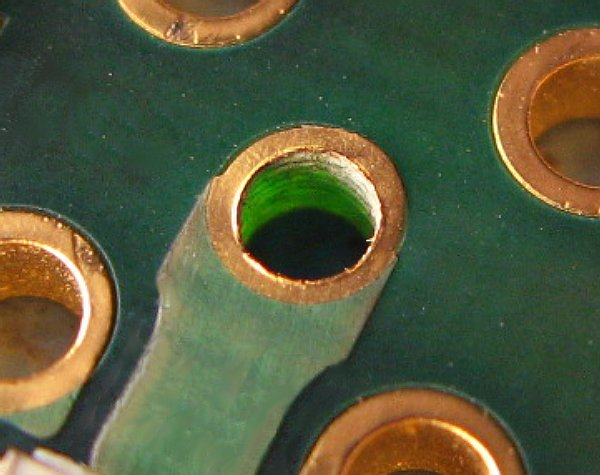
\includegraphics[width=.5\textwidth]{Figures/through_hole_correcto}
	\caption{Via con galvanización correcto en un PCB}
	\label{fig:thr_correcto}
\end{figure}

\begin{figure}[h]
\centering
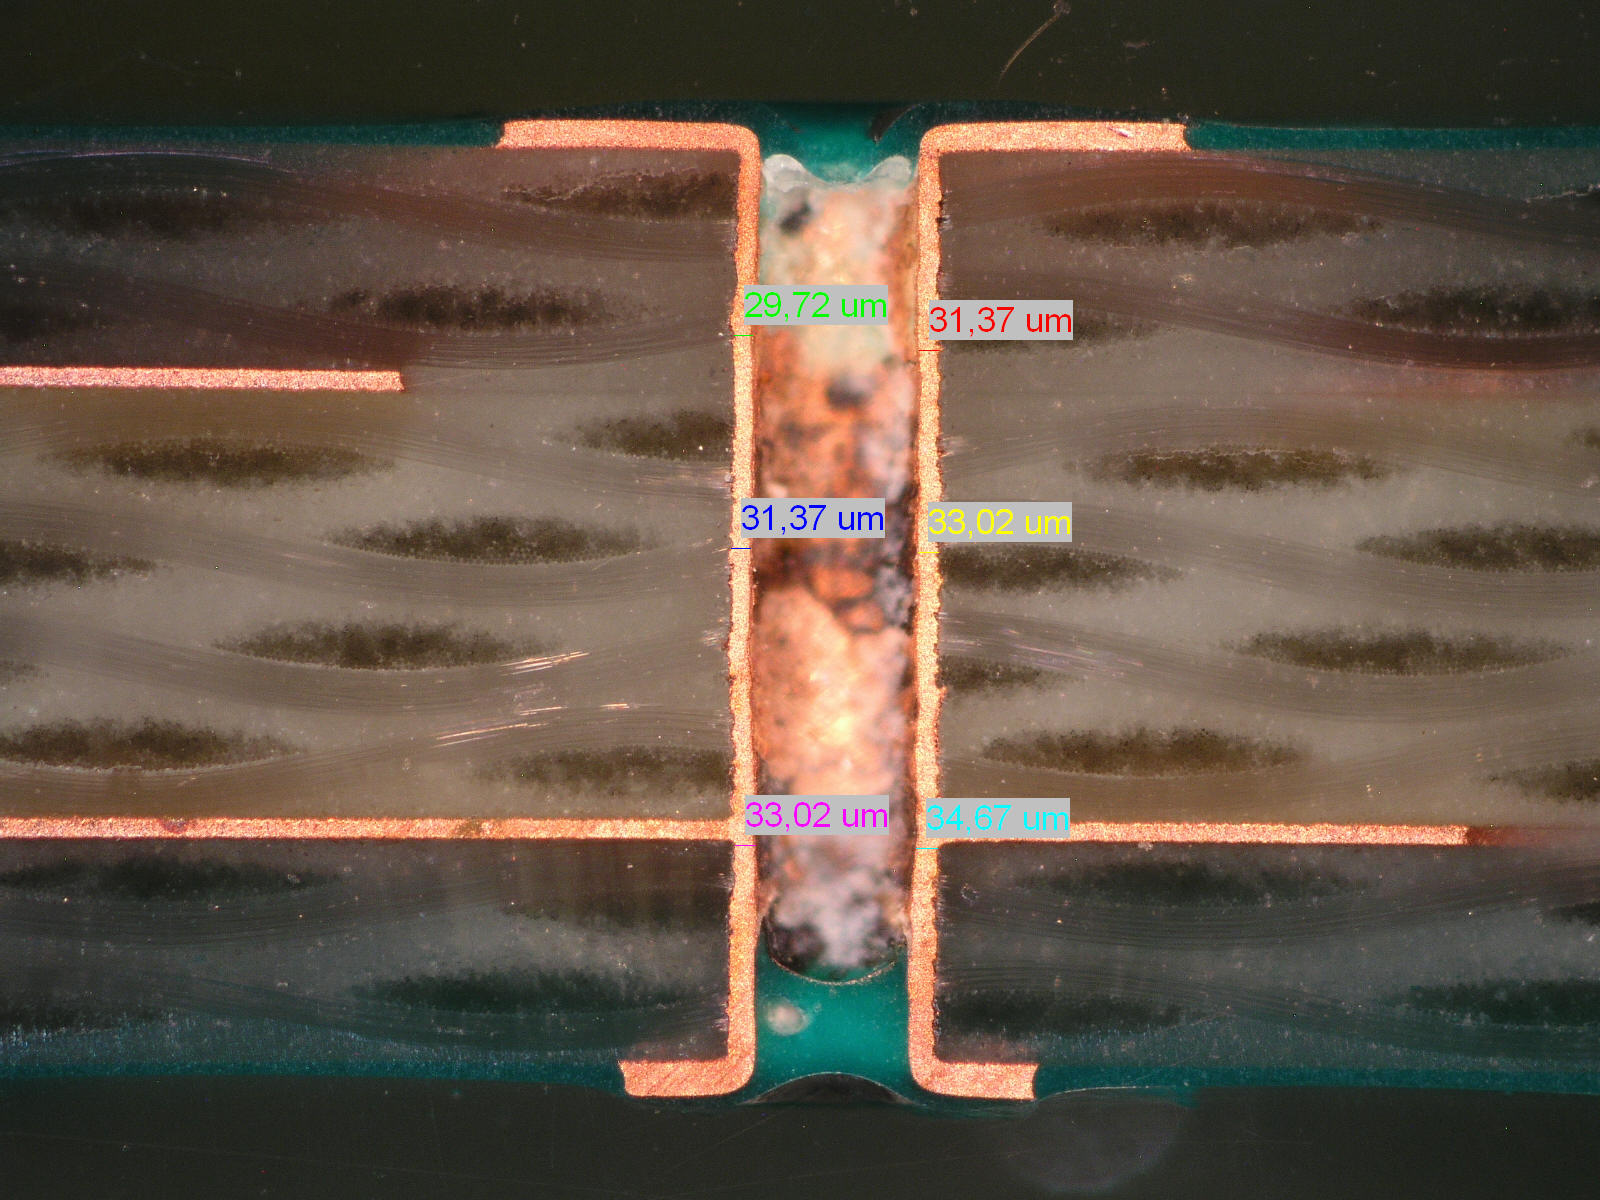
\includegraphics[width=.5\textwidth]{Figures/through_hole_perfil}
\caption{Perfil de una via correctamente galvanizada}
	\label{fig:thr_correcto_perfil}
\end{figure}

Cuando este proceso no ocurre correctamente se originan distintas fallas, donde las más comunes son: vías sin galvanizar, vías obstruidas por exceso de cobre y capa no uniforme de metal cobre en la vía con riesgo de no conductividad. En la Figura \ref{thr_incorrecto_perfil} se observan las distintos grosores de cobre en vias mal galvanizadas en función de su ubicación en el sustrato del PCB.

\begin{figure}[h]
	\centering
	\includegraphics[width=.8\textwidth]{Figures/through_hole_perfil_fallado}
	\caption{Perfil un conjunto de sustratos con vías mal galvanizadas}
	\label{fig:thr_incorrecto_perfil}
\end{figure}

El proceso requiere una sucesión de baños por distintas soluciones químicas y enjuagues en agua, previas y después del proceso de electrolisis con cobre sobre el sustrato. En la Figura \ref{fig:diagrama_proceso} se resumen los pasos de forma simplificada, en el proceso de PCB se utilizan mas de 10 etapas.

\begin{figure}[h]
	\centering
	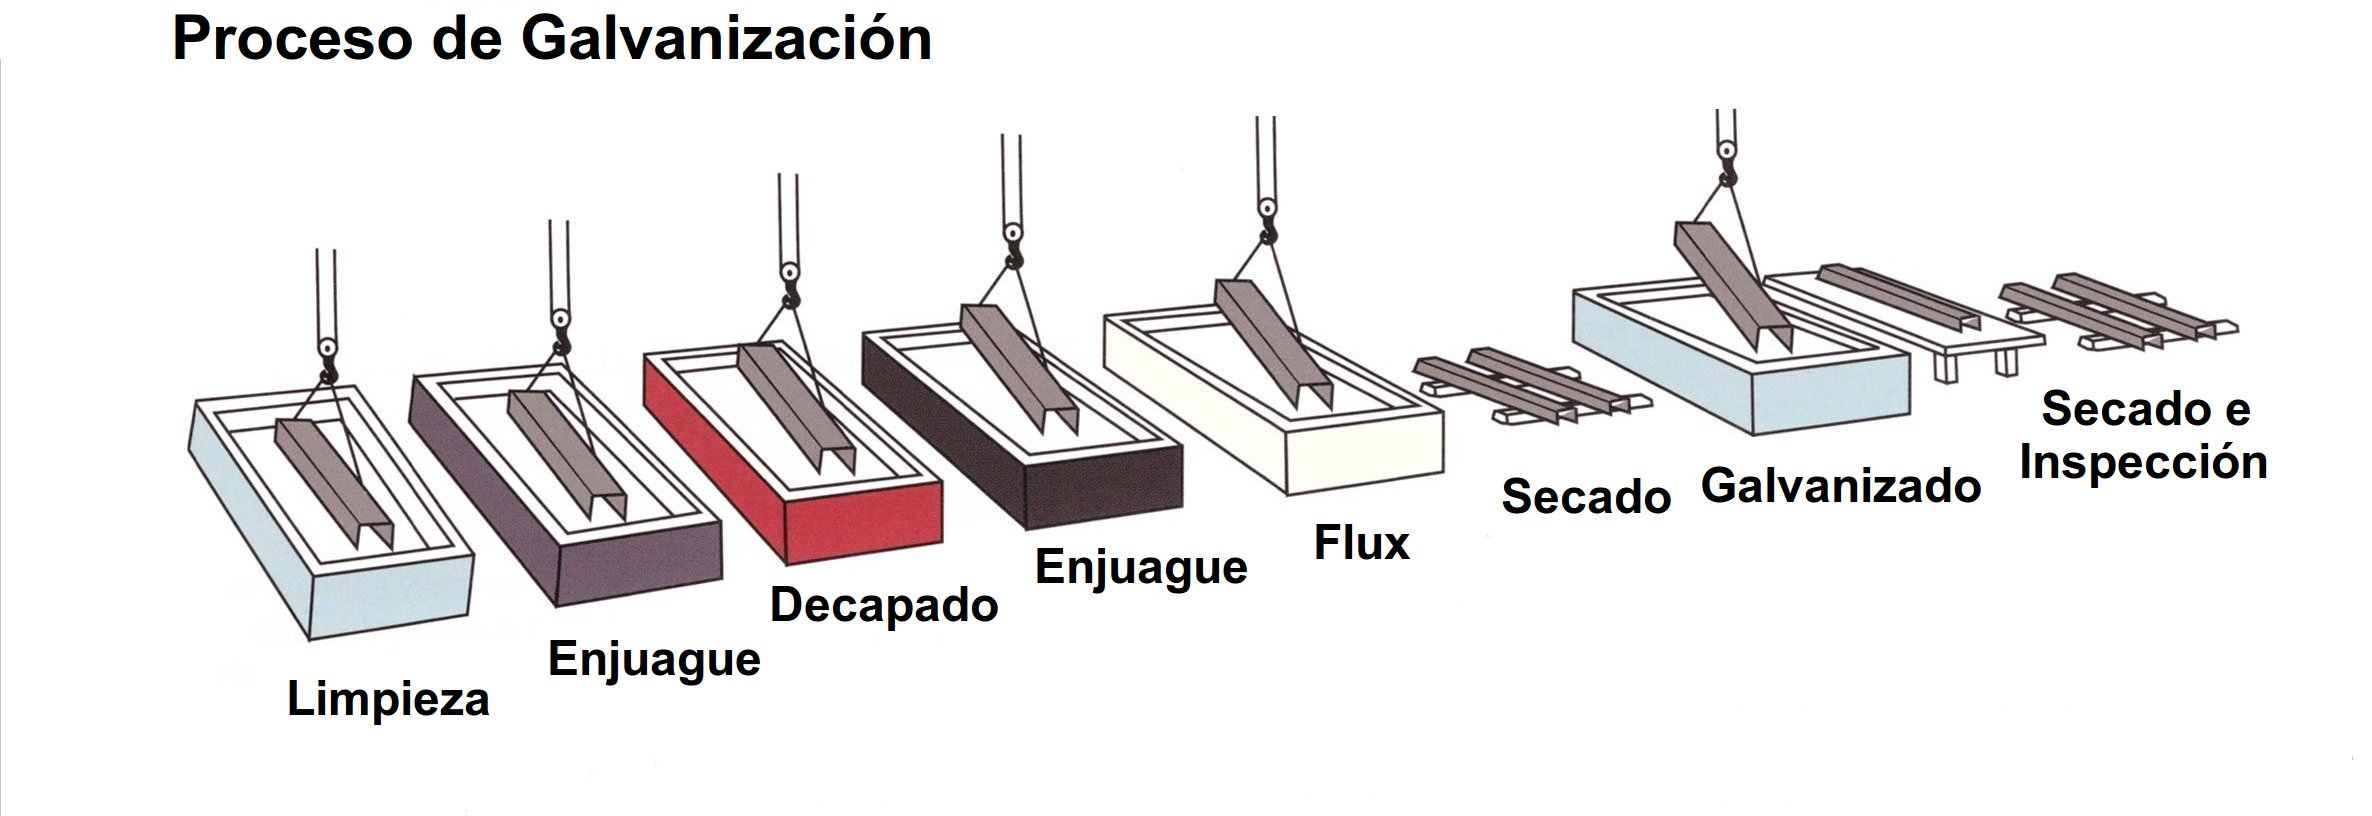
\includegraphics[width=.8\textwidth]{Figures/diagrama_galvanizado_castellano}
	\caption{Diagrama simplificado de una linea de galvanizado}
	\label{fig:diagrama_proceso}
\end{figure}


\LaTeX{} no es \textsc{WYSIWYG} (What You See is What You Get), a diferencia de los procesadores de texto como Microsoft Word o Pages de Apple o incluso LibreOffice en el mundo open-source. En lugar de ello, un documento escrito para \LaTeX{} es en realidad un archivo de texto simple, llano que \emph{no contiene formato} . Nosotros le decimos a \LaTeX{} cómo deseamos que se aplique el formato en el documento final escribiendo comandos simples entre el texto, por ejemplo, si quiero usar \emph{texto en cursiva para dar énfasis}, escribo \verb|\emph{texto}| y pongo el texto en cursiva que quiero entre medio de las llaves. Esto significa que \LaTeX{} es un lenguaje del tipo \enquote{mark-up}, muy parecido a HTML.

\section{Motivación y objetivo}

A partir de la búsqueda de incrementar los niveles de calidad en producto final surgió la necesidad de agregar control y monitoreo a determinadas bateas criticas en el proceso de modo de asistir a los operarios de planta en tiempo real sobre alguna anomalía en los parámetros antes de continuar con el proceso. En la Figura \ref{fig:planta_actual} se puede ver como es la linea de proceso actual.

\begin{figure}[h]
	\centering
	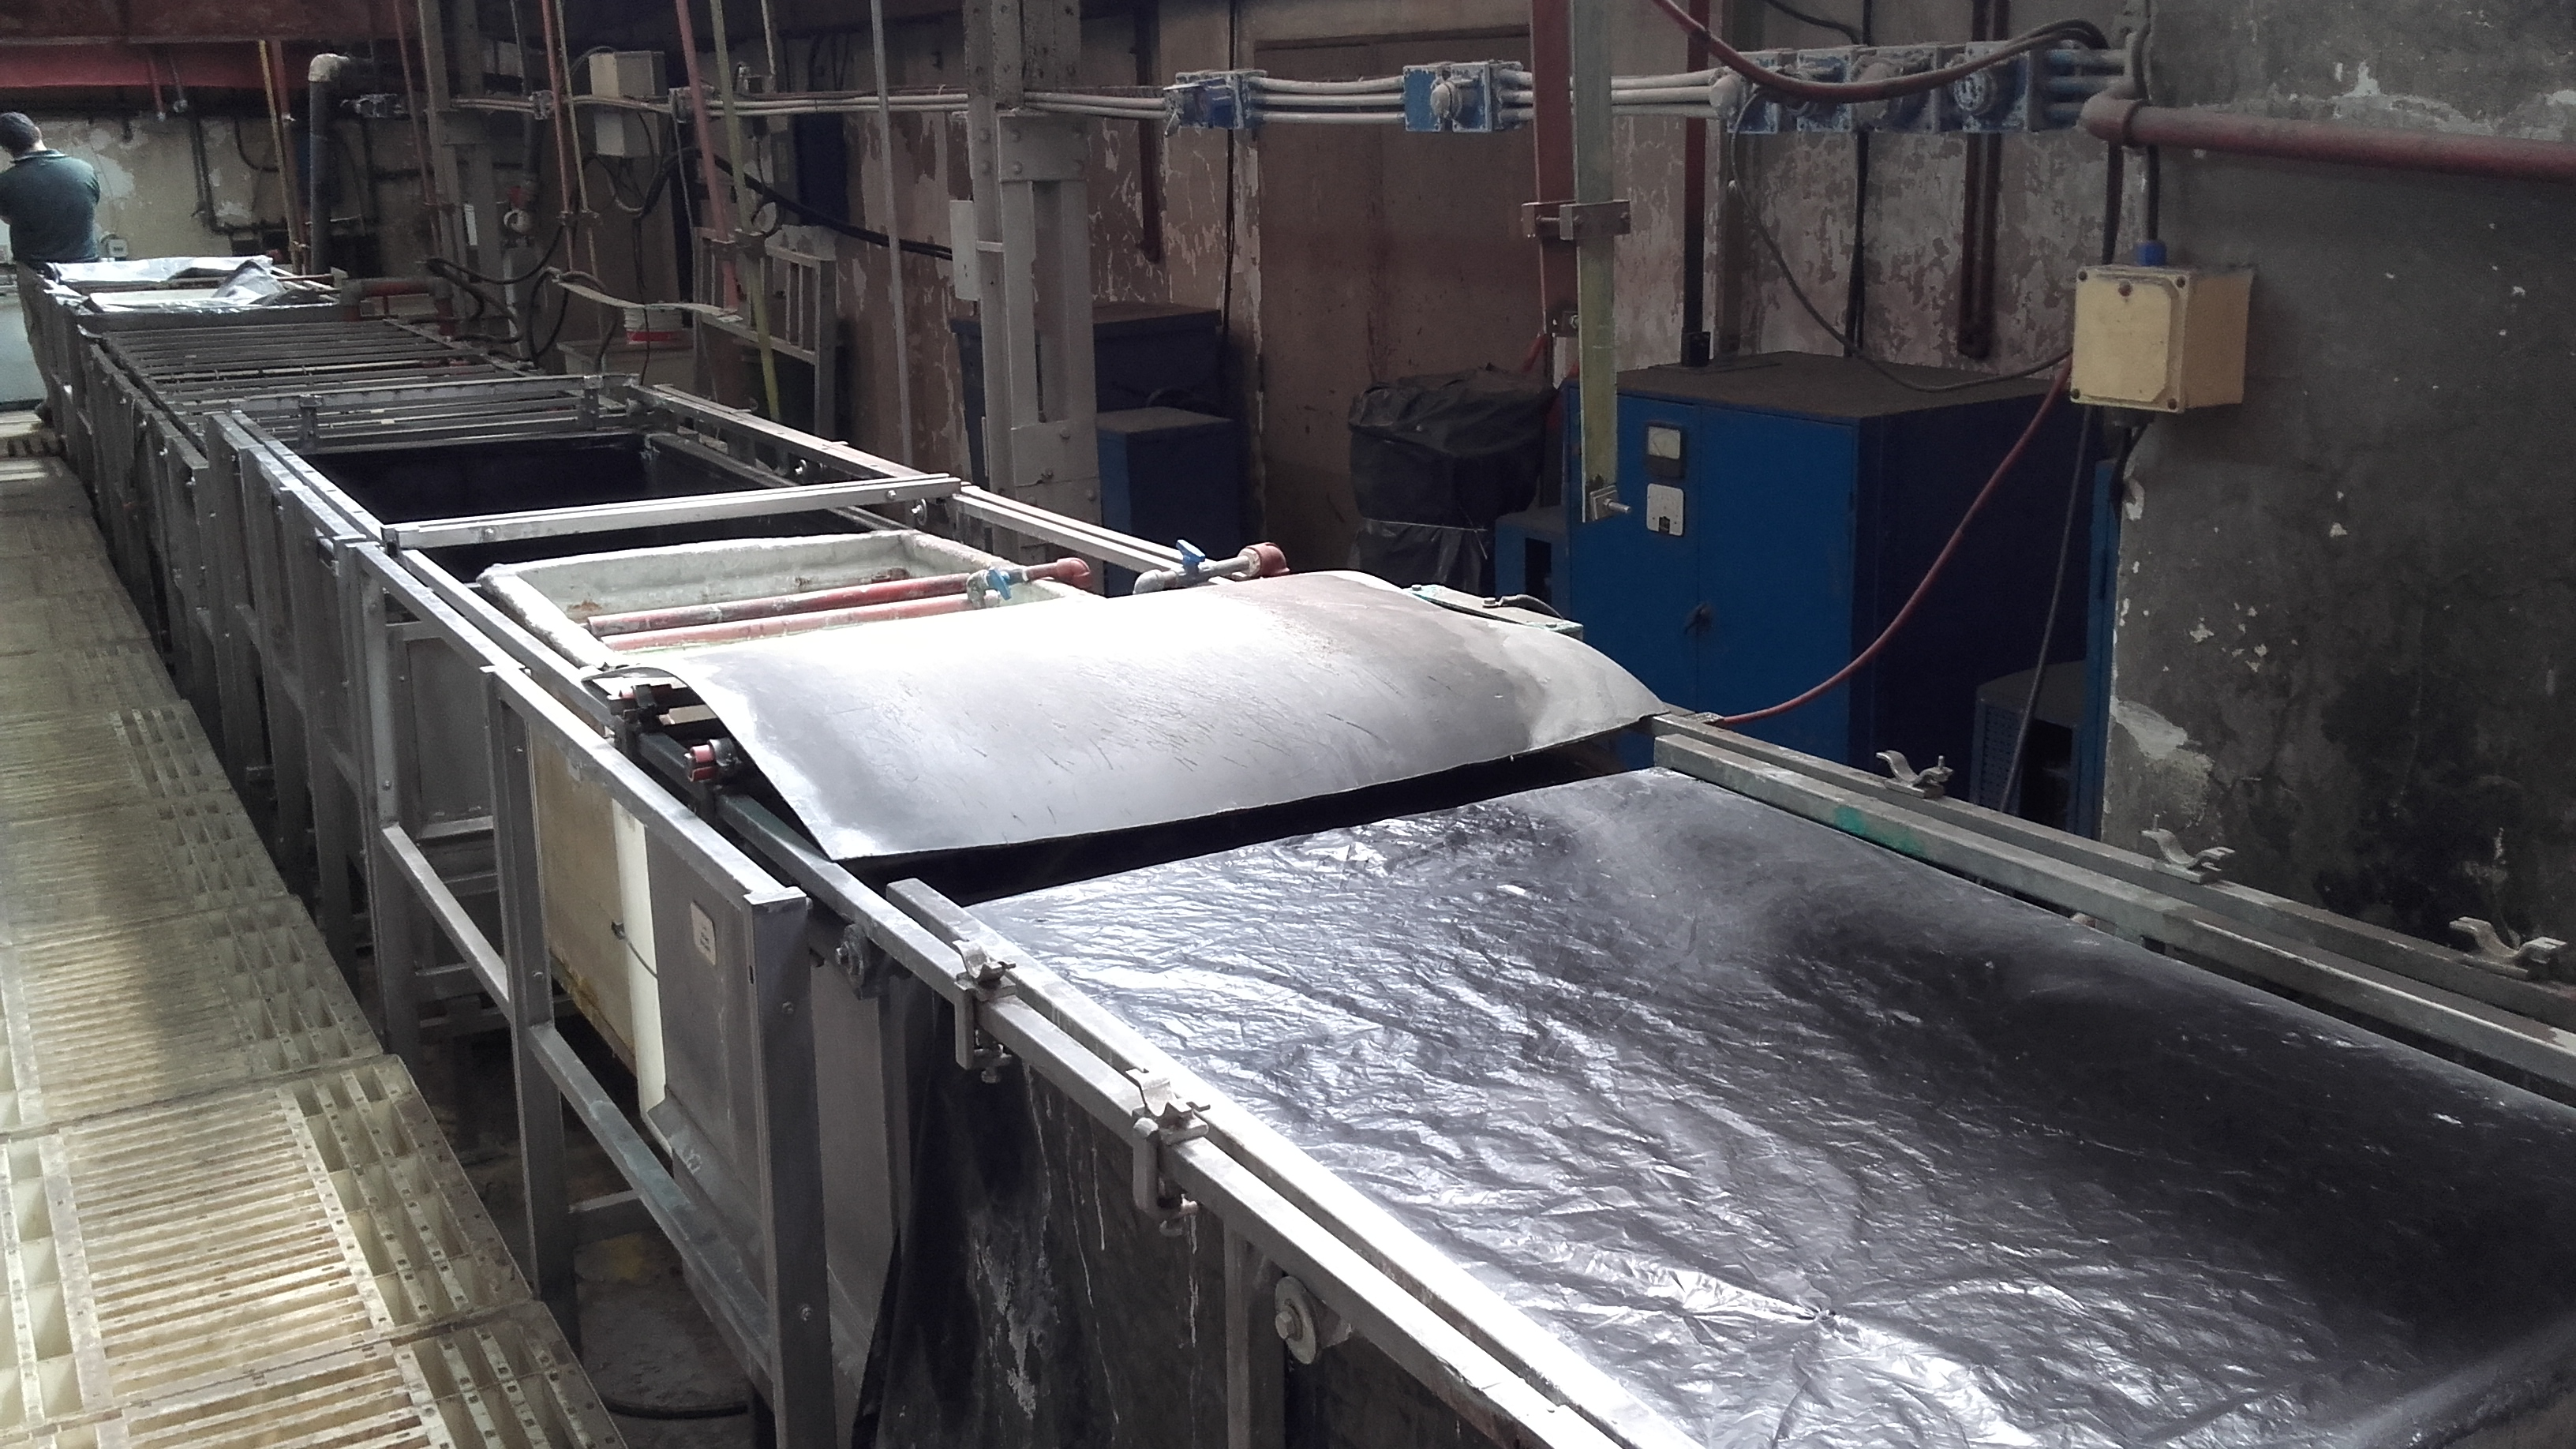
\includegraphics[width=.8\textwidth]{Figures/planta_actual}
	\caption{Linea de galvanizada actual operada manualmente}
	\label{fig:planta_actual}
\end{figure}

Como segundo objetivo como el proceso actual es totalmente hecho a mano y se esta trabajando en modernizarla y cambiarla de lugar se busca que el mismo sistema pueda integrar a una linea de traslación de los PCBs automatizada, lo cual se logró con el conteo de tiempo de posicionamiento por etapa.  

Finalmente a modo de control general y auditoría se necesitaba que el sistema registre los valores de las parámetros de medición en archivos . 

Si usted es nuevo a \LaTeX{}, hay un muy buen libro electrónico - disponible gratuitamente en Internet como un archivo PDF - llamado, \enquote{A (not so short) Introduction to \LaTeX{}}. El título del libro es generalmente acortado a simplemente \emph{lshort}. Puede descargar la versión más reciente en inglés (ya que se actualiza de vez en cuando) desde aquí:
\url{http://www.ctan.org/tex-archive/info/lshort/english/lshort.pdf}

Está disponible en varios idiomas además del inglés. Se puede encontrar la versión en español en la lista en esta página: \url{http://www.ctan.org/tex-archive/info/lshort/}


\section{Objetivo}

El presente sistema embebido se focalizó en la confiabilidad, robustez y adaptabilidad con las interfaces eléctricas necesarias para que funcione en un ambiente industrial con los actuadores y sensores determinados por el cliente. Para tal fin se propuso que el mismo funcione sobre la plataforma eduCIAA en conjunto con una placa de interfaz hecha a medida, como un prototipo de prueba previo al desarrollo de un hardware propio.

\subsection{Alcance}

El proyecto incluyó los siguientes puntos:
\begin{itemize}
	\item Estudio preliminar de las arquitecturas adecuadas para la implementación del sistema principal y subsistemas.
	\item Diseño de alto nivel (arquitectura) del sistema.
	\item Diseño del sistema en lenguaje C para plataforma CIAA.
	\item Plan de pruebas unitarias y ensayos (testbenchs) para cada subsistema.
	\item Plan de pruebas de integración y ensayos (testbenchs) para agrupaciones de subsistemas.
	\item Plan de pruebas del sistema y ensayos (testbenchs) para el sistema completo.
	\item Documentación del sistema y subsistemas que incluye:
	\begin{enumerate}
		\item Descripción de entradas y salidas (frecuencias, tamaño y tipos de datos, señales de control, etc.)
		\item Descripción de parámetros del sistema.
		\item Requerimientos funcionales implementados trazables a los requerimientos del proyecto (matriz de trazabilidad).
		\item Hipótesis de diseño, justificación de la elección del diseño, estudios previos y marco teórico.
		\item Diagrama de arquitectura.
		\item Reporte de ensayos realizados.
		\item Referencias bibliográficas.
	\end{enumerate}
	\item Análisis y construcción del banco de pruebas.
\end{itemize}

El proyecto no incluyó: 
\begin{itemize}
	\item Estudio de los sensores y actuadores, se basará dicha información en los datos dados por el cliente. 
	\item Análisis de mejor solución para implementación de sistema de reporte remoto de variables y registros históricos. 
	\item Test del sistema en lugar de producción. La planta se encontraba en reestructuración y modernización.
\end{itemize}



%----------------------------------------------------------------------------------------

\section{Utilizando esta plantilla}

Si usted está familiarizado con \LaTeX{}, entonces puede explorar la estructura de directorios de esta plantilla y proceder a personalizarla agregando su información en el bloque \emph{INFORMACIÓN DE LA PORTADA} en el archivo \file{memoria.tex}.  

Se puede continuar luego modificando el resto de los archivos siguiendo los lineamientos que se describen en la sección \ref{sec:FillingFile} en la página \pageref{sec:FillingFile}.

Asegúrese de leer el capítulo \ref{Chapter2} acerca de las convenciones utilizadas para las Memoria de los Trabajos Finales de la Carrera de Especialización en Sistemas Embebidos de FIUBA.

Si es nuevo en \LaTeX{} se recomienda que continue leyendo el documento ya que contiene información básica para aprovechar el potencial de esta herramienta.

Si usted está escribiendo un documento con mucho contenido matemático, entonces es posible que desee leer el documento de la AMS (American Mathematical Society) llamado, \enquote{A Short Math Guide for \LaTeX{}}. Se puede encontrar en línea en el siguiente link: \url{http://www.ams.org/tex/amslatex.html} en la sección \enquote{Additional Documentation} hacia la parte inferior de la página.



\subsection{Acerca de esta plantilla}

Esta plantilla \LaTeX{} está basada originalmente en torno a un archivo de estilo \LaTeX{} creado por Steve R.\ Gunn de la  University of Southampton (UK), department of Electronics and Computer Science. Se puede encontrar su trabajo original en el siguiente sitio de internet:
\url{http://www.ecs.soton.ac.uk/~srg/softwaretools/document/templates/}

El archivo de Gunn, \file{ecsthesis.cls} fue posteriormente modificado por Sunil Patel quien creó una plantilla esqueleto con la estructura de carpetas. El template resultante se puede encontrar en el sitio web de Sunil Patel:
\url{http://www.sunilpatel.co.uk/thesis-template}

El template de Patel se publicó a través de  \url{http://www.LaTeXTemplates.com} desde donde fue modificado muchas veces en base a solicitudes de usuarios. La versión 2.0 y subsiguientes representan cambios significativos respecto a la versión de la plantilla modificada por Patel, que es de hecho, dificilmente reconocible. El trabajo en la version 2.0 fue realizado por Vel Gayevskiy y Johannes Böttcher.

Uno de los primeros graduados de la Carrera de Especialización en Sistemas Embebios de la UBA, el Ing. \href{mailto:pbos@fi.uba.ar}{Patricio Bos} modificó los contenidos de la versión 2.3 para crear una plantilla altamente adaptada a la Carrera de Especialización de la UBA.

%----------------------------------------------------------------------------------------







\chapter{ Introducción Específica } % Main chapter title
%----------------------------------------------------------------------------------------
%	INTRODUCCION
%----------------------------------------------------------------------------------------
Aquí se abordan con mas detalle el proceso de fabricación, los parámetros críticos y las fallas que pueden derivarse. Luego se exponen los criterios de diseño del prototipo a partir de los casos de uso del mismo, modos de funcionamiento. Finalmente se detalla la lista de requerimientos completos, a saber: funcionales y no funcionales, de interfaz, de diseño y futuros.

\section{ Galvanizado de circuitos impresos }

El proceso de galvanizado consiste en adherir a un objeto metálico una delgada capa de otro metal, de unos pocos micrones de espesor. Este material le otorga mejores propiedades al objeto como ser conductividad eléctrica, mayor resistencia mecánica o resistencia a la corrosión. 

Los métodos para lograrlos pueden ser diversos. Entre los mas comunes están el baño químico y por electrólisis. El método químico es utilizado generalmente en estructuras con superficies homogéneas y consiste en sumergir el producto dentro de un baño con el metal galvanizante en forma de solución química o bien a alta temperatura, incluyendo algunas etapas de pre- acondicionado. La figura \ref{fig:galvanizado_quimico} es un diagrama simplificado de método químico.
El método electrolítico insume un gran consumo de energía eléctrica y mas etapas de pre-tratamiento de la superficie, pero tiene la ventaja de ser mas controlable el grosor del galvanizado, se suele hacer a temperatura ambiente y es mas versátil para aplicar sobre superficies no metálicas con un pre acondicionado previo. En la figura \ref{fig:galvanizado_electrolitico} se  un proceso electrolítico donde básicamente el objeto recibe distintos pre-tratamientos para preparar la superficie antes y después del efecto electrolítico. 

\hspace{1px}
\begin{figure}[h]
	\centering
	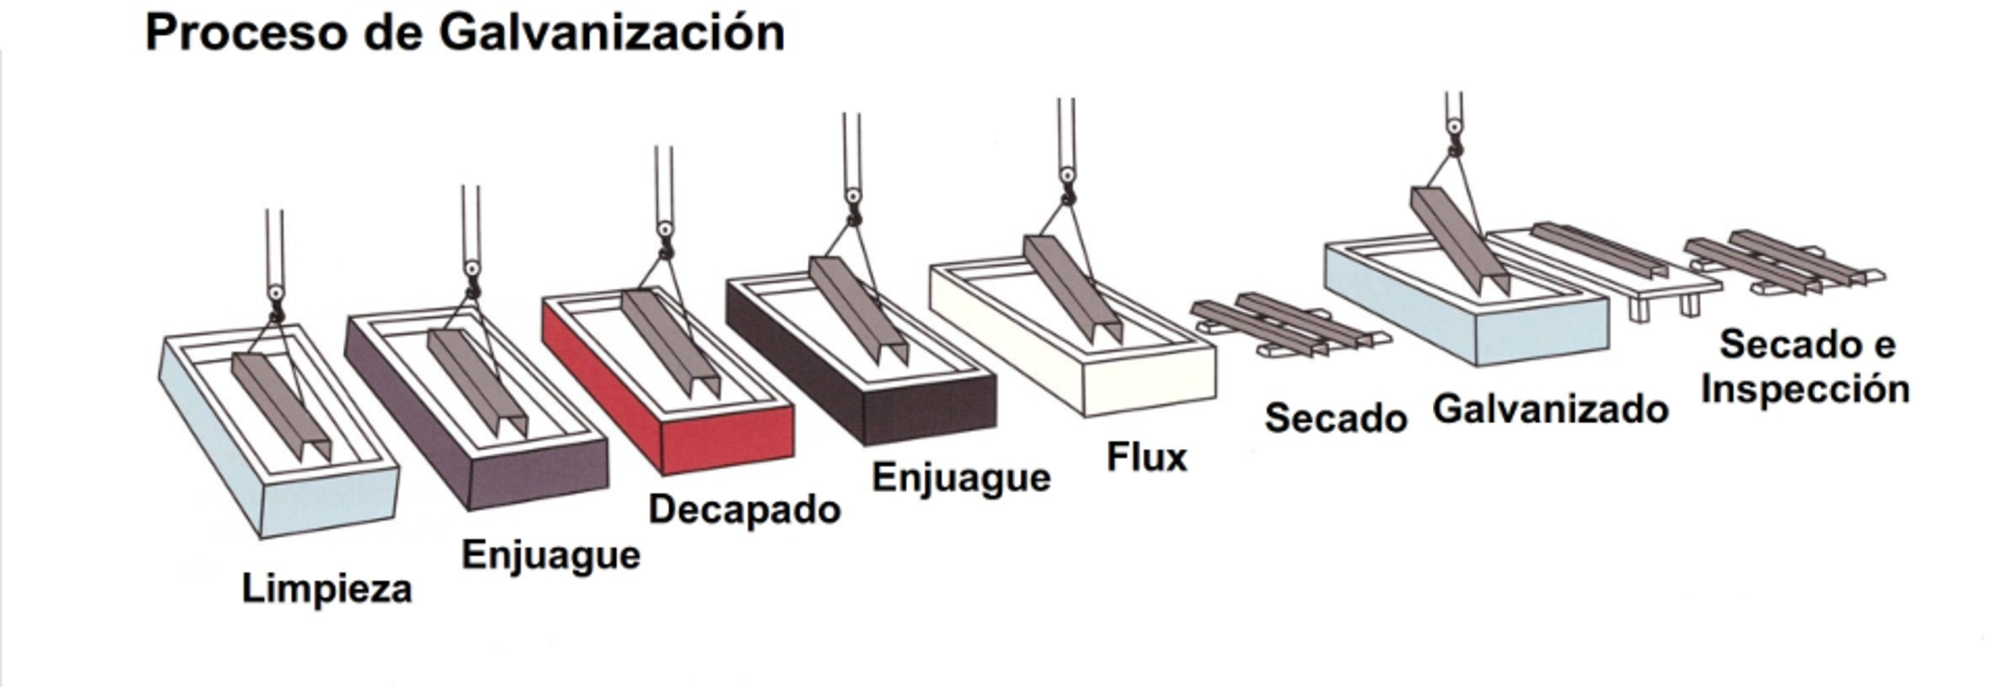
\includegraphics[width=1.0\textwidth]{Figures/Cap_2/diagrama_galvanizado_basico}
	\caption{Proceso de galvanizado químico a través de la inmersión del objeto en distintos baños químicos.}
	\label{fig:galvanizado_quimico}
\end{figure}
\hspace{1px}
\begin{figure}[h]
	\centering
	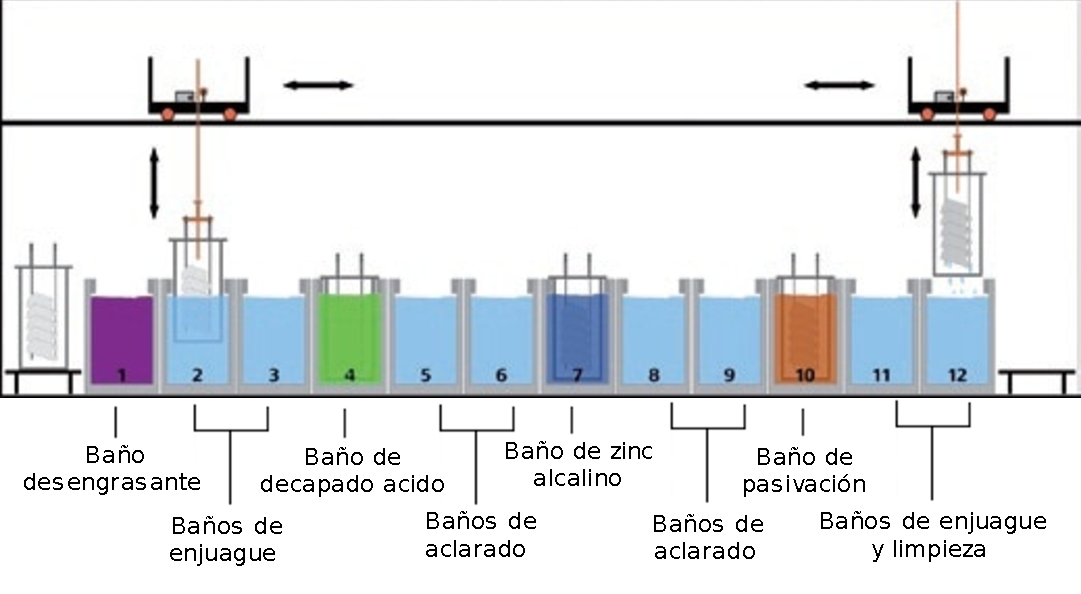
\includegraphics[width=1.0\textwidth]{Figures/Cap_2/diagrama_galvanizado_electrolitico}
	\caption{Proceso de galvanizado electrolítico a través de la inmersión del objeto en distintos baños químicos.}
	\label{fig:galvanizado_electrolitico}
\end{figure}

La forma utilizada en las placa de circuito impreso (PCB) es a través de la electrólisis del objeto dentro de una solución con sales metálicas, con una fuente de muy alta corriente continua de bajo voltaje, mas bloques del metal necesario para el galvanizado. En la figura \ref{fig:copper_electroplating} se muestra un caso donde el ánodo es de cobre y el cátodo es el PCB a galvanizar. 

\begin{figure}[h]
	\centering
	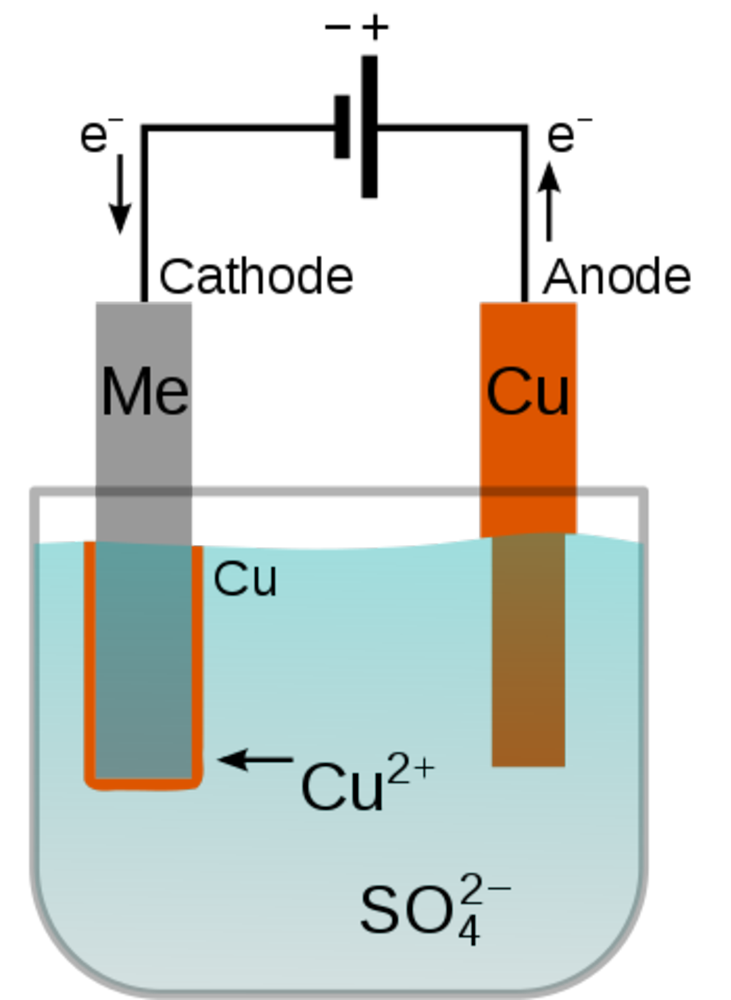
\includegraphics[width=0.3\textwidth]{Figures/Cap_2/galvanizado_copper_electroplating}
	\caption{Proceso electrolítico a través del cual se fija la capa de material sobre la superficie del objeto.}
	\label{fig:copper_electroplating}
\end{figure}


\subsection{ Proceso de galvanizado por electrólisis }

En la fabricación de PCBs se parte de un material base de sustrato de laminas epoxi FR4 revestido con laminas de cobre. Este debe ser sometido previo a realizar la electrólisis en sí, a una sucesión de baños químicos para limpiar y homogeneizar toda las partes metálicas de superficie. El proceso es repetido con variantes del metal galvánico para lograr el circuito final. 

En el proceso de fabricación de un PCB se utilizan aproximadamente 10 etapas distintas entre dos procesos. El primer proceso incluye el galvanizado con cobre de las vías entre capas, sobre el material laminado previamente perforado. El segundo proceso incluye el grabado del circuito impreso en si, previamente fijada la imagen negativa sobre las superficies del mismo.
Existe una similitud en muchos de los pasos de inmersión de las placas en los productos químicos, que resulta en controlar mismos parámetros en las distintas cubas a lo largo del proceso. 
En la Figura \ref{fig:diagrama_proceso} se muestra los efectos producidos sobre un perfil de una vía en un sustrato FR4, para las etapas mas relevantes.

\begin{figure}[h]
	\centering
	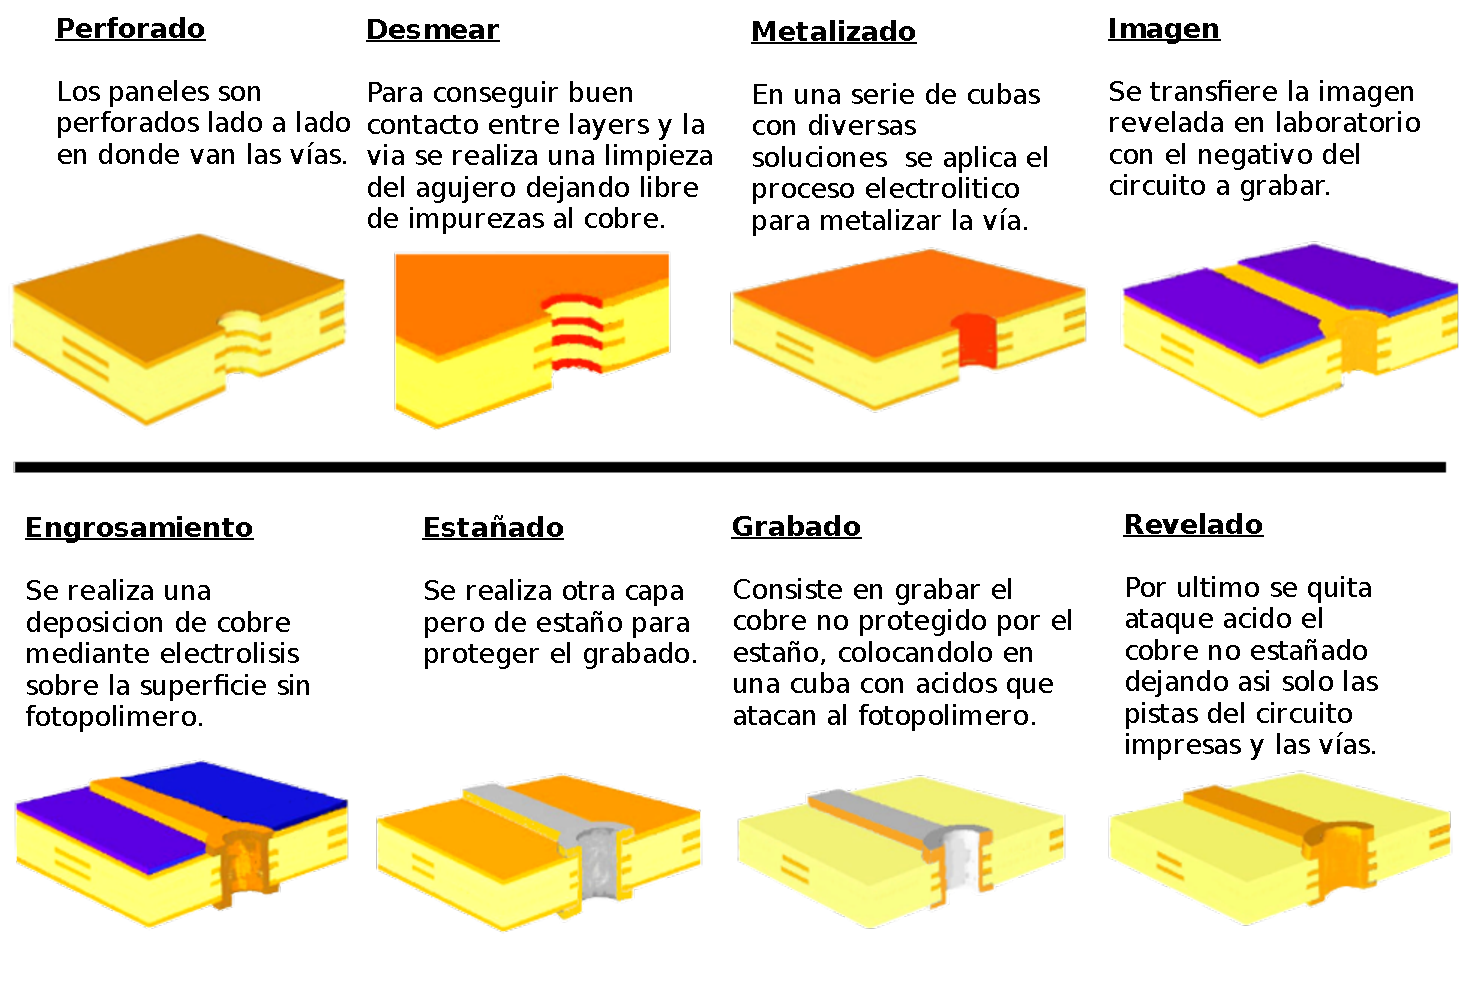
\includegraphics[width=1.0\textwidth]{Figures/Cap_2/diagrama_galvanizado_completo}
	\caption{ Diagrama simplificado de las etapas \footnotemark. \footnotemark.}
	\label{fig:diagrama_proceso}
\end{figure}

\footnotetext{\url{https://www.4pcb.com/media/presentation-how-to-build-pcb.pdf}} 
\footnotetext{SASE2013-Circuitos Impresos de Marcos Mayer} 

En el proceso desarrollado en Daichi S.A. la serie completa, desde que se cortan los paneles FR4 hasta que se coloca la mascara antisoldante, incluye entre 20 a 25 de pasos los cuales se resumen a continuación lo mas importantes.
% Agregar una TABLA con los pasos segun etapa a grandes rasgos.
% *************************************************************************

La figura \ref{fig:galvanizado_pcb} muestra el resultado final de un PTH (Plated Through Hole o agujero pasante metalizado) o  vía, de un un PCB.
\begin{figure}[h]
	\centering
	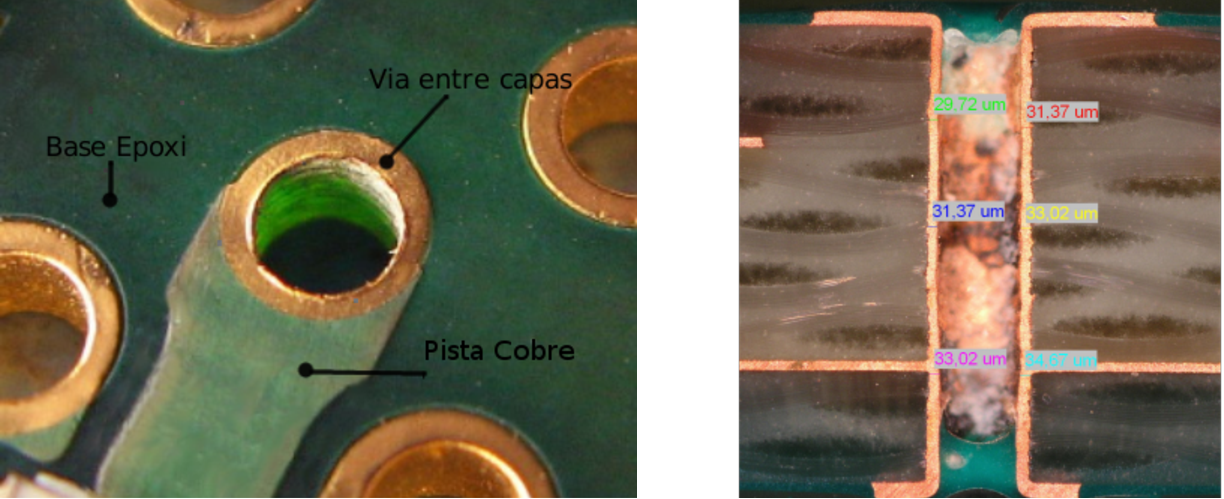
\includegraphics[width=.8\textwidth]{Figures/Cap_2/galvanizado_pcb_2}
	\caption{Vía entre capas galvanizada en un PCB}
	\label{fig:galvanizado_pcb}
\end{figure}

\section{ Parámetros críticos del galvanizado }

En el proceso de galvanización de PCBs el control de ciertos parámetros físicos-químicos en cada una de las etapas es fundamental para garantizar la uniformidad y calidad del baño metálico. 

En las diferentes bateas de la linea de galvanizado es necesario controlar, según cada etapa uno o algunos de los siguientes parámetros físicos-químicos del proceso:
\begin{itemize}
	\item Temperatura.
	\item Nivel de líquidos.
	\item Conductividad o concentración de iones.
	\item Corriente entregada (electrólisis).
	\item Inyección de aire.
\end{itemize}

Actualmente en la linea de galvanizado los operadores cuentan solo con su experiencia y con el soporte de instrumental de medición básico que poseen en algunas las etapas de la linea. Para saber cuando una etapa esta finalizada se basan en el tiempo que saben funciona y por observación del estado del proceso. Esto puede acarrear muchos problemas si no se han estandarizado procesos. Además es causante de que el producto final muchas veces no tenga una calidad estándar y de que no se puedan prevenir fallas del proceso a tiempo.
 
Por todo esto para saber cuando un proceso fue realizado correctamente, es necesario tener información precisa, detallada y respetar los tiempos e indicadores preestablecidos para lograr el tipo de galvanizado buscado. 

\subsection{ Fallas en el galvanizado de PCBs }

En la producción de PCBs el resultado final correcto es aquel en donde el espesor del baño metálico es uniforme en toda la superficies y paredes de las vías. Cuando este proceso no ocurre correctamente se originan distintas fallas, de las cuales las más comunes son:
\begin{itemize}
	\item Vías sin galvanizar.
	\item vías obstruidas por exceso de cobre.
	\item Laminado no uniforme de metal cobre.
	\item Micro cortes del cobre y puntos de no conductividad.
\end{itemize}

En la figura \ref{fig:thr_incorrecto_perfil} se observan las distintos grosores de cobre con vías mal galvanizadas en función de su ubicación en el sustrato del PCB y la cercanía al ánodo de cobre.

\begin{figure}[h]
	\centering
	\includegraphics[width=.9\textwidth]{Figures/Cap_2/through_hole_perfil_fallado}
	\caption{Perfil de vías según la ubicación relativa en los sustratos y el los cátodos.}
	\label{fig:thr_incorrecto_perfil}
\end{figure}

En la figura \ref{fig:fallas_en_PTH} se observa los problemas originados por la mala preparación previa de las superficies metálicas del sustrato, originado puntos sin continuidad o circuitos abiertos que lo volverán no aptos para la producción de circuitos.

\begin{figure}[h]
	\centering
	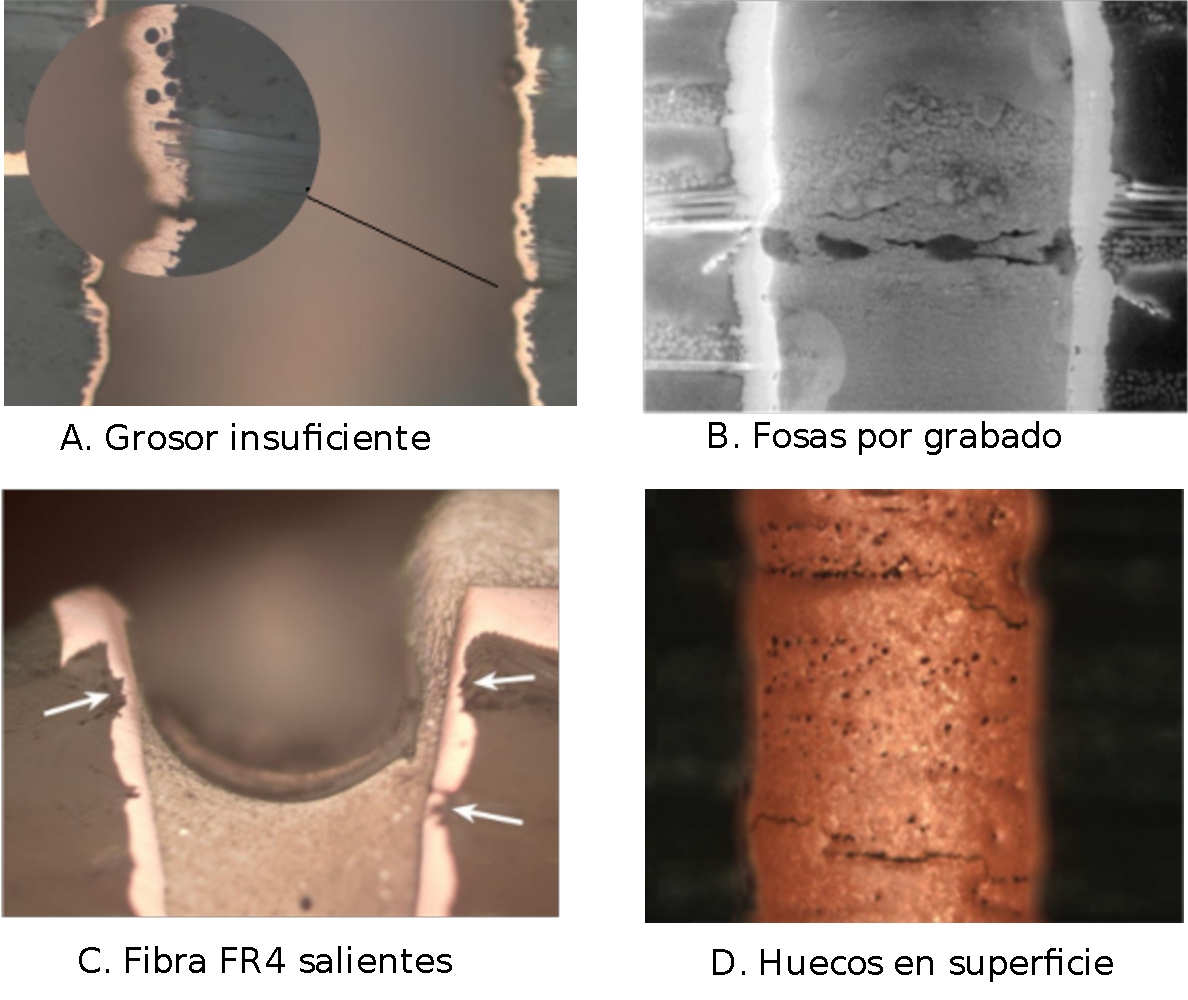
\includegraphics[width=.8\textwidth]{Figures/Cap_2/fallas_en_PTH}
	\caption{ Las capas de cobre se alejan del borde del orificio.}
	\label{fig:fallas_en_PTH}
\end{figure}

\section{ Determinación de la solución a utilizar } 

A fin de lograr recopilar los detalles de la arquitectura del sistema desarrollado, es necesario primero definir y determinar casos de uso, requerimientos técnicos y definiciones generales originados por la nueva planta, su operación y las necesidades del cliente. 

\subsection{ Definiciones Generales }

La linea cuenta con varias etapas en forma consecutiva independientes entre si pero con parámetros característicos similares, se determinó implementar un solo prototipo capaz de procesar el conjunto de parámetros del proceso, capaz de interactuar con los distintos usuarios del entorno y configurable según las etapas a monitorear.

El sistema debe funcionar entonces en modo predeterminado según los distintos escenarios posibles dentro de las etapas del proceso. De esta manera con un mismo hardware mas los sensores y actuadores necesarios, se puede supervisar y controlar las partes del proceso que se crean necesarias. En la figura \ref{fig:banco_pruebas} se muestra la implementación del banco de prueba que se diseño para la validación del prototipo.

\begin{figure}[h!]
	\centering
	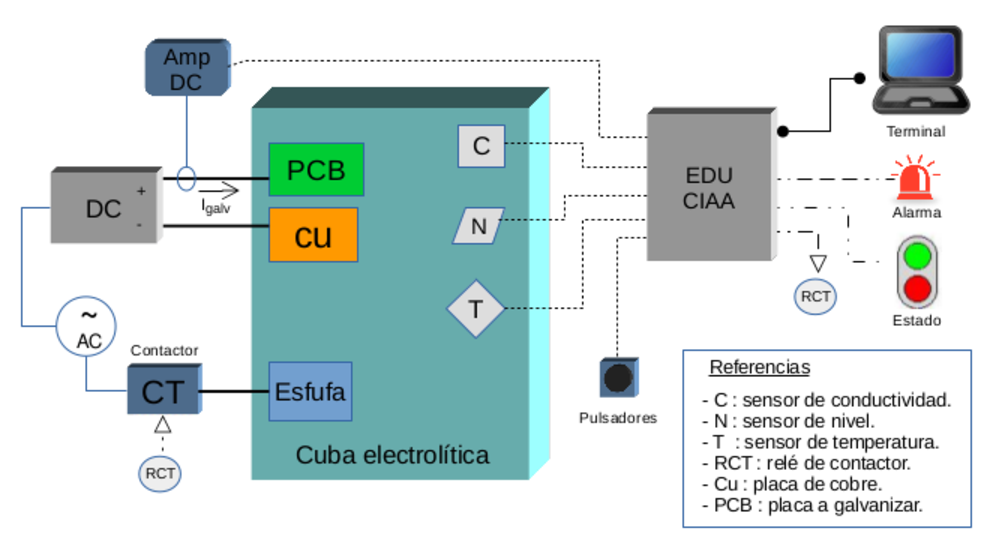
\includegraphics[width=1.2\textwidth]{Figures/Cap_2/diagrama_prototipo}
	\caption{Banco de pruebas de validación del prototipo. }
	\label{fig:banco_pruebas}
\end{figure}

En una etapa posterior luego de la validación del prototipo el cliente desarrollará un hardware a medida para usar en su planta. El mismo será producido en las cantidades necesarias según el numero de etapas que se determinen. Por ultimo estos distintos módulos funcionarán de manera independiente entre si.

% AGREGAR UNA IMAGEN DEL PROTOTIPO QUE SE PENSABA CONSTRUIR Y COMO SE PROBARIA A MODO DE BOSQUEJO.


\subsection{ Casos de Uso }
\label{subsec:casos_de_uso}
Los casos de uso del sistema se definen para determinar como se vincula éste con los distintos usuario, en función del modo de funcionamiento posible. Estos quedan entonces predeterminados por los escenarios posibles que se pueden originar en la operación de la linea. Los casos mas relevantes son:

\begin{enumerate}
	\item Puesta en alta y configuración del dispositivo, usado por personal técnico.
	\item Puesta en marcha en modo de funcionamiento 1, usado por el operario y el técnico.
	\item Puesta en marcha en modo de funcionamiento 2, usado por el operario y el técnico.
\end{enumerate}

Los modos 1 y 2 se refieren a dos configuraciones a partir de los escenarios mas comunes de conexión del prototipo. A fin de simplificar la puesta en marcha en campo y por la limitación de numero de entradas analógicas de la EDU-CIAA.
En la tabla \ref{modos_funcionamiento} se observa un resumen de los periféricos involucrados en cada caso.

%TABLA ****************
\begin{table}[h!]
\begin{flushleft}
\begin{tabular}{|m{1,2cm}|m{4cm}|m{4cm}|m{4cm}|} \hline
{\textbf{Modo}} & {\textbf{Función}} & {\textbf{Entradas}} & {\textbf{Salidas}}\\ \hline
{\textit{Func 1}} & {Controla nivel, temperatura, conductividad del liquido en la cuba.} & { Nivel tanque, temperatura del liquido, conductividad del liquido.} & {Contactor calefactor, contactor válvula de recambio, alarma de estado.} \\ \hline
{\textit{Func 2}} & {Controla nivel, temperatura, energía consumida en la cuba.} & {Nivel tanque, temperatura del liquido, corriente entrante.} & {Contactor calefactor, contactor válvula de recambio, alarma de estado.} \\ \hline
{\textit{Config.}} & {Modifica pines asignados, valores de alarma, tiempos de muestreo.} & {Comandos por terminal de pc.} & {Confirmación por terminal de pc y leds.} \\ \hline
\end{tabular}
\end{flushleft}
\caption{Descripción modos de funcionamiento.}
\label{modos_funcionamiento}
\end{table}

En la Figuras \ref{fig:casoUsoAlta} y \ref{fig:casodeUso1y2} se notan las interacciones entre los distintos submódulos del sistema en función de los casos de usos y los usuarios vinculados.

\begin{figure}[h!]
	\centering
	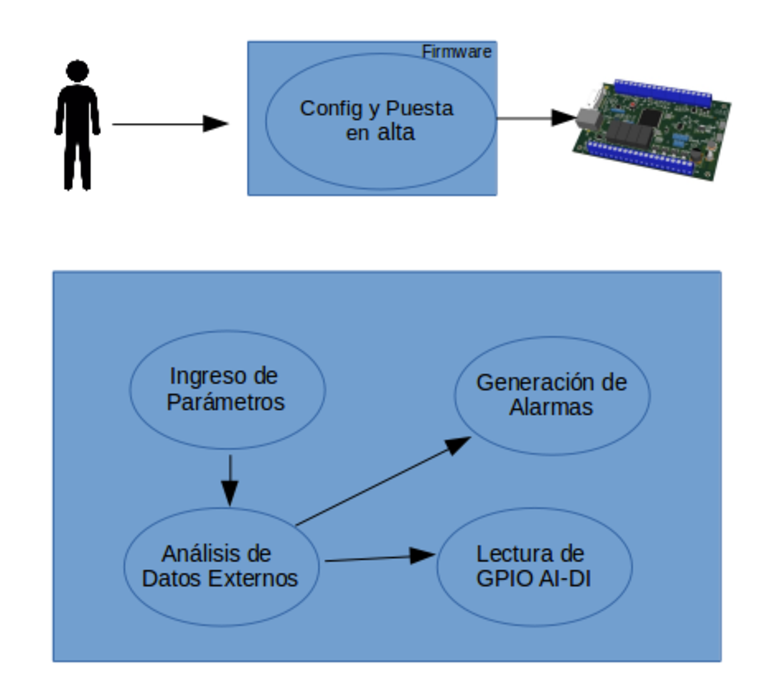
\includegraphics[width=.9\textwidth]{Figures/Cap_2/caso_uso_Alta_UML}
	\caption{Diagrama UML caso de uso de puesta en alta.}
	\label{fig:casoUsoAlta}
\end{figure}

La puesta en alta es el momento en que se determinan a través de la interfase terminal HMI (Humman Machine Interface o interfase hombre maquina) las parámetros a medir y configuraciones de los puertos del hardware.

\begin{figure}[h!]
	\centering
	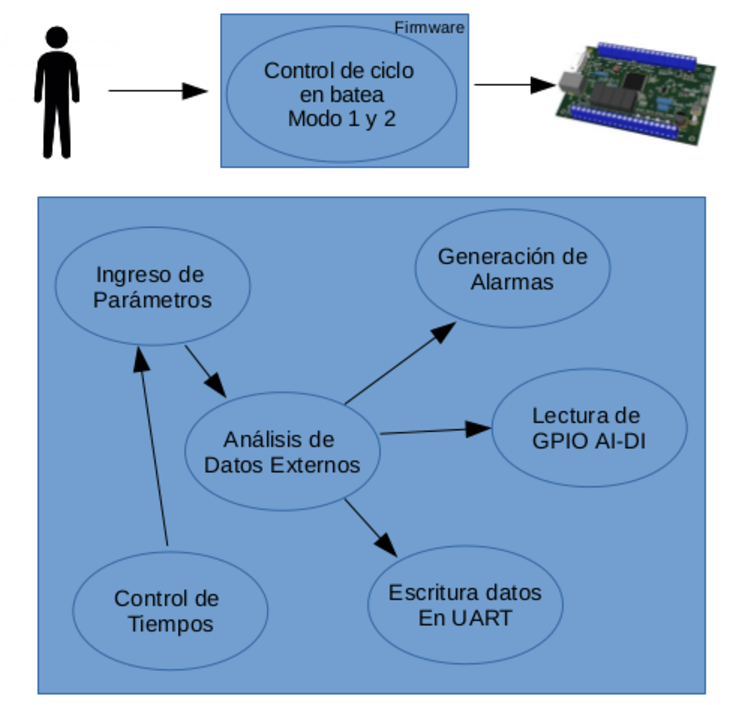
\includegraphics[width=.8\textwidth]{Figures/Cap_2/caso_uso_Marcha_UML}
	\caption{Diagrama UML de casos de uso Modo 1 y 2.}
	\label{fig:casodeUso1y2}
\end{figure}

En el Apéndice \ref{AppendixA} se detallan la secuencias involucradas en cada una de los casos de uso.

\subsection{ Requerimientos funcionales y no funcionales }
\label{subsec:Requerimientos}

A continuación se enumera lista completa con los requerimientos surgidos del análisis en conjunto con el personal de la planta tanto del problema, los casos uso y las prestaciones que tendrá la nueva planta. 
Cabe mencionar que la lista de requerimientos se originó previamente en la materia \emph{Gestión de Proyectos} del posgrado.

\begin{enumerate}
%------------------------------------------------------------------------
\item Requerimientos Funcionales
\begin{enumerate}

\item Temperatura (RFTEM)
\begin{enumerate}
\item El sistema medirá la temperatura con un resolución de XX, cada YY segundos.
\item El sistema mantendrá la temperatura controlada según los parámetros configurados por el usuario.
\item El sistema elevará la temperatura a través de la activación de una salida digital conectada a una resistencia.
\item La activación de la resistencia se implementará a través de una ventana Smith Trigger para evitar la intermitencia y generación de ruido en las líneas de alimentación principal. Cruce por 0.
\item En caso de que la temperatura se exceda de rango de considerar interrumpir el proceso y emitir una alarma.
\item El sistema almacenará al menos XX valores de temperatura en un archivo en memoria flash.
\end{enumerate}

\item Energía (RFENE)
\begin{enumerate}
\item El software medirá la corriente total (DC) entregada al proceso de electrólisis cada XX segundos, con YY de resolución.
\item El software medirá la tensión aplicada (DC) entre los bornes del electrólisis cada XX segundos con YY de resolución.
\item El sistema almacenará al menos XX valores de corriente y tensión en un archivo en memoria flash.
\item Los rangos de valores óptimos de tensión y corriente serán tomados de los parámetros de lote ingresados por el usuario y mostrados por pantalla para su configuración manual en la fuente de alimentación principal.
\end{enumerate}

\item Conductividad (RFCOND)
\begin{enumerate}
\item El software calculará a través de la corriente y tensión medidas en el tanque de galvanización, la conductividad de la solución salina cada XX segundos con YY de resolución.
\item El software deberá compensar las eventuales desviaciones de la conductividad óptima a través de la activación de XX válvulas de aditivos.
\end{enumerate}

\item Interfaces Hombre-Máquina (RFHMI)
\begin{enumerate}
\item El sistema contará con una pantalla estado del sistema con variables a definir.
\item El sistema contará con un método de ingreso de parámetros de lote a procesar.
\item Deberá permitir ingresar parámetros en modo manual y otros en modo codificado.
\item Deberá brindar a través de una interfaz Ethernet los históricos almacenados en memoria flash de variables del proceso que necesiten ser auditadas tras una etapa o tras el proceso completo. El máximo de registros será de XX número de puntos en formato YY.
\end{enumerate}

\item Tiempos (RFTI)
\begin{enumerate}
\item El software llevará un conteo del tiempo entre cada baño en las bateas, desde el momento que se inicia hasta el final del proceso.
\item En cada etapa deberá avisar y esperar a que un operario habilite la iniciación de la siguiente etapa.
\end{enumerate}

\item Niveles de bateas (RFNB)	
\begin{enumerate}
\item Evaluará que los niveles dentro del galvanizador estén dentro de los rangos permitidos de operación.
\item En caso de algún nivel crítico se emitirán alarmas y se considera la interrupción del proceso.
\end{enumerate}

\end{enumerate}

%------------------------------------------------------------------------
\item Requerimientos de Interfaz
\begin{enumerate}

\item Temperatura (RITEM)
\begin{enumerate}
\item La temperatura será medida a través de un sensor analógico de tolerancia XX.
\item La temperatura se medirá en los tanques XX, lo que arroja un total de YY numero de entradas analógicas independientes.(+xxAI)
\end{enumerate}

\item Energía (RIENE)
\begin{enumerate}
\item Tendrá un sensor de alta corriente del tipo XX conectado en una entrada analógica, para la corriente de galvanizador. (+1AI)
\item Tendrá un sensor de tensión de tipo XX conectados a los bornes de galvanizador. (+1AI)
\end{enumerate}

\item Conductividad (RICOND)
\begin{enumerate}
\item Tendrá XX dispositivos dosificador/es conectados a salidas digitales. (+xxDO)
\end{enumerate}

\item Interfaces Hombre-Máquina (RIHMI)
\begin{enumerate}
\item Debe mostrar información a través de un puerto VGA/HDMI con una taza de refresco menor a XX segundos. (+1USB)
\item Tomará de una entrada serie USB los valores de lote. (+1USB)
\item Accionara a través de una salida digital una alarma sonora/lumínica en caso de algún tipo de falla. (+1DO, +1AO) 
\item Contará con uno o dos pulsadores a fin de poder detener y accionar el procesos de galvanización, conectados a una/dos entradas binarias.(+1/2DO)
\item Dispondrá de una conexión remota a través de Ethernet. (+1ETH)
\end{enumerate}

\item Niveles de bateas (RINB)
\begin{enumerate}
\item Tendrá XX sensores de nivel conectados a entradas digitales. (+xxDI)
\end{enumerate}

\end{enumerate}

%------------------------------------------------------------------------
\item Requerimientos no Funcionales (RNF)
\begin{enumerate}
\item Deberá ser probada la funcionalidad a través de un banco de pruebas que se ajuste al comportamiento del sistema. 
\end{enumerate}
%------------------------------------------------------------------------
\item Restricciones de Diseño (RD)
\begin{enumerate}
\item De los requerimientos de interfaz se resume que como mínimo el hardware deberá contar con las siguientes interfaces:\\
- Entradas analógicas (AI) >= 3	\\
- Entradas digitales (DI) >= 3	\\
- Salidas analógicas (AO) >= 1	\\
- Salidas digitales (DO) >= xx	\\
- Puerto USB (USB) = 2	\\
- Puerto RED (ETH) = 1	\\
\end{enumerate}
%------------------------------------------------------------------------
\item Requerimientos a Futuro (RAF)
\begin{enumerate}
\item Brindar información acerca de si es necesario realizar una limpieza de sistema. Se puede utilizar como parámetro el número de procesos que se ejecutaron 	 	 	
\item Deberá permitir loguearse antes de iniciar el proceso, así tener un responsable de operación.
\item Deberá interactuar con una cinta de transportación automática que llevará las placas de una batea a otra. Accionara los motores (paso a paso?) de transporte y de elevación.
\item Si no se respetan los tiempos el sistema deberá dejar asentado el técnico y las acciones manuales ejecutadas a fin de tener un histórico antes posibles fallas en el lote.
\end{enumerate}

\end{enumerate}

En función de estos se propuso implementar el proyecto sobre una plataforma EDU-CIAA \citep{CIAA} en conjunto con una placa de interfaz hecha a medida. 
Los parámetros definidos con XX son aquellos que no pudieron ser definidos en su momento con el cliente ¿?
Los RFHMI relacionados con el ingreso de lotes no pudieron implementarse en esta primer etapa del proyecto al no tener un sistema centralizado que controle las etapas.







 
\definecolor{mygreen}{rgb}{0,0.6,0}
\definecolor{mygray}{rgb}{0.5,0.5,0.5}
\definecolor{mymauve}{rgb}{0.58,0,0.82}

\lstset{ %
  backgroundcolor=\color{white},   % choose the background color; you must add \usepackage{color} or \usepackage{xcolor}
  basicstyle=\footnotesize,        % the size of the fonts that are used for the code
  breakatwhitespace=false,         % sets if automatic breaks should only happen at whitespace
  breaklines=true,                 % sets automatic line breaking
  captionpos=b,                    % sets the caption-position to bottom
  commentstyle=\color{mygreen},    % comment style
  deletekeywords={...},            % if you want to delete keywords from the given language
  %escapeinside={\%*}{*)},          % if you want to add LaTeX within your code
  %extendedchars=true,              % lets you use non-ASCII characters; for 8-bits encodings only, does not work with UTF-8
  %frame=single,	                   % adds a frame around the code
  keepspaces=true,                 % keeps spaces in text, useful for keeping indentation of code (possibly needs columns=flexible)
  keywordstyle=\color{blue},       % keyword style
  language=[ANSI]C,					% the language of the code
  %otherkeywords={*,...},           % if you want to add more keywords to the set
  numbers=left,                    % where to put the line-numbers; possible values are (none, left, right)
  numbersep=5pt,                   % how far the line-numbers are from the code
  numberstyle=\tiny\color{mygray}, % the style that is used for the line-numbers
  rulecolor=\color{black},         % if not set, the frame-color may be changed on line-breaks within not-black text (e.g. comments (green here))
  showspaces=false,                % show spaces everywhere adding particular underscores; it overrides 'showstringspaces'
  showstringspaces=false,          % underline spaces within strings only
  showtabs=false,                  % show tabs within strings adding particular underscores
  stepnumber=1,                    % the step between two line-numbers. If it's 1, each line will be numbered
  stringstyle=\color{mymauve},     % string literal style
  tabsize=2,	                   % sets default tabsize to 2 spaces
  title=\lstname,                   % show the filename of files included with \lstinputlisting; also try caption instead of title
  morecomment=[s]{/*}{*/}%
}



\chapter{Diseño e Implementación} % Main chapter title
\label{Chapter3} % Change X to a consecutive number; for referencing this chapter elsewhere, use \ref{ChapterX}
%----------------------------------------------------------------------------------------
%	SECTION 1
%----------------------------------------------------------------------------------------
Aquí se presenta el detalle del hardware planteado como un \enquote{poncho} sobre la EDU-CIAA, y la interfaz con los elementos de la planta. Luego se describe la estructura lógica del software con detalles del diseño sobre diagramas de interacción entre tareas, diagramas de capas y otras consideraciones relevantes del código.


\section{Análisis del Hardware}
\label{analisis_hardware}
El prototipo se implemento sobre una EDU-CIAA en conjunto con un hardware de adaptación de las interfaces. Para ello se utilizaron los proyectos de código abierto Kicad \citep{kicad} para la elaboración del poncho de la EDU-CIAA \citep{brengiponchos} que adapta las entradas y salidas de los conectores de expansión con los sensores y actuadores utilizados en la planta. 

\subsection{ Sensores y actuadores }

% Aca van todo lo referido a consideraciones importantes sobre los esquematicos.
%\subsubsection{Esquemáticos del prototipo final}

Para la adaptación de las interfaces con termocuplas y termistores se necesitaron circuitos de adaptación de señal. Para el primer caso se uso un circuito integrado compensador de juntura debido a la alinealidad en la respuesta de ese tipo de sensores. Para ello se eligió el MAX31855KASA+ \footnotemark como una solución simplificadora. 
También existen soluciones implementadas con amplificadores multietapas que son mas económicos pero que obligan a implementar la transducción de la señal en el microprocesador \citep{interOpamp}.\\
En la Figura \ref{fig:cirCompTermocupla} se observa una configuración típica de adaptación para termocupla.

\footnotetext{\url{bucar la url con la hoja de datos}} 

\begin{figure}[h!]
	\centering
	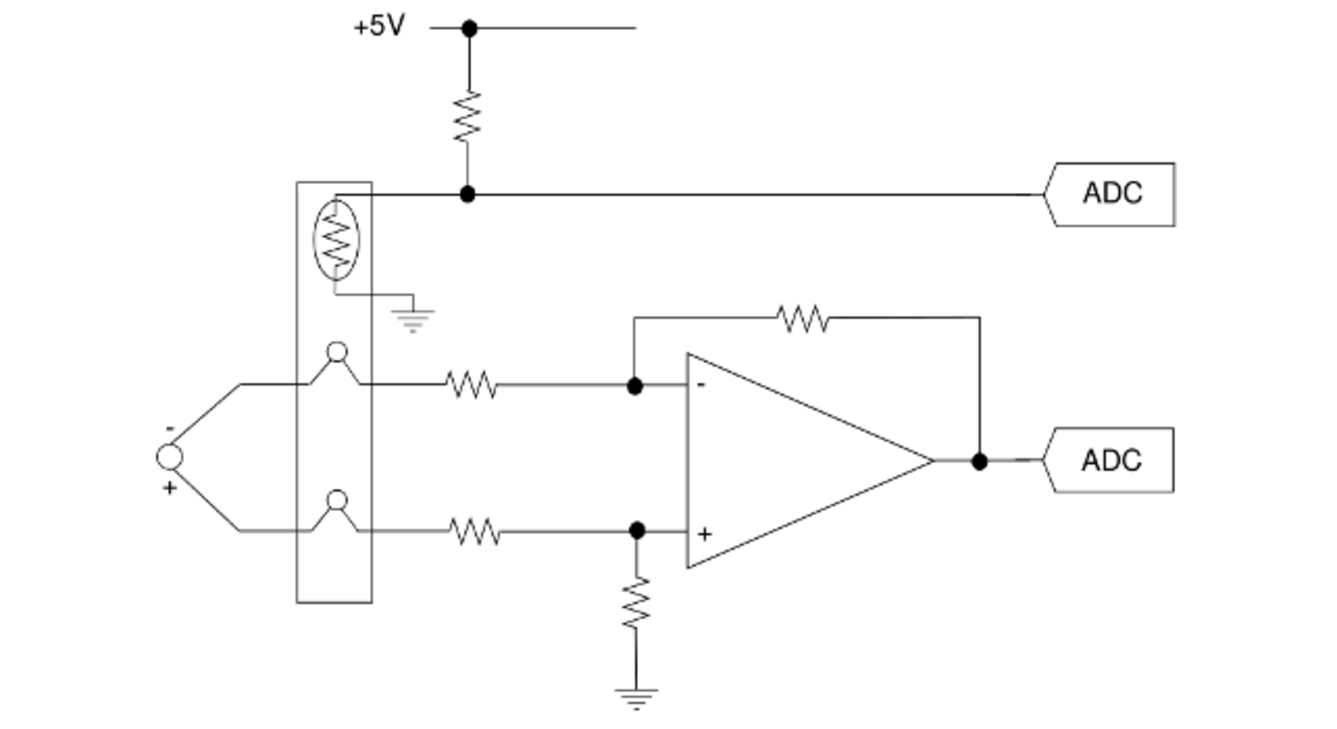
\includegraphics[width=.7\textwidth]{Figures/Cap_3/circuito_ampl_termocupla}
	\caption{Circuito simplificado de amplificación y compensación de termocuplas.}
	\label{fig:cirCompTermocupla}
\end{figure}

En el caso del termistor el circuito de adaptación es mas simple debido a que señal obtenida es prácticamente lineal y solamente es necesario amplificar a los niveles de trabajo de la entrada analógica del procesador. En la Figura \ref{fig:cirCompTermistor} se observa en tipo de circuito que se implementó.

\begin{figure}[h!]
	\centering
	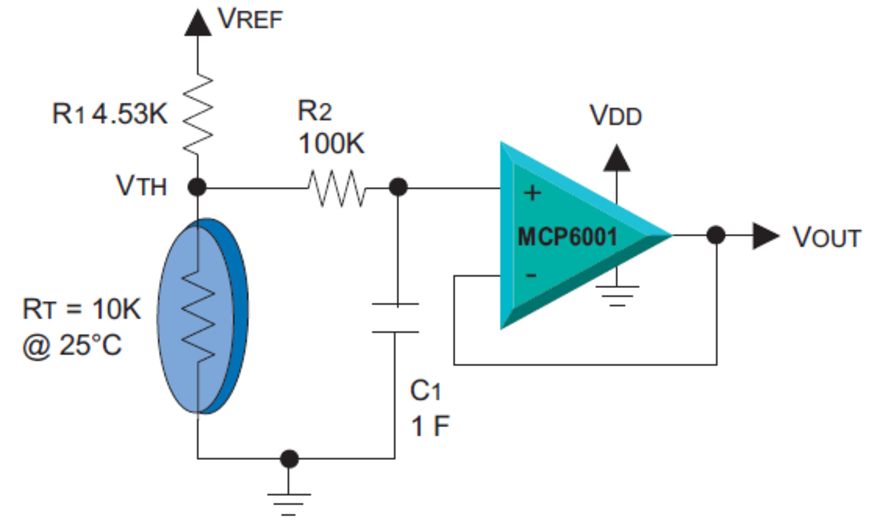
\includegraphics[width=.7\textwidth]{Figures/Cap_3/thermistor-conventional-circuit}
	\caption{Circuito simplificado de amplificación y compensación de termistores.}
	\label{fig:cirCompTermistor}
\end{figure}

En el caso de la medición de corriente y tension continua para las pruebas solo se consideraron sensores de baja potencia a fin de poder validar el comportamiento. Cabe aclarar que en linea de producción las fuentes de galvanizado son de muy alta potencia y la intensidad es leída actualmente con pinzas amperímetros AC/DC.
La medición de tension se toma en principio con un circuito aislado con foto-transistores para obtener mayor aislación de la fuente de corriente.
La medición de continuidad o salinidad del agua se resolvió implementarla con un circuito de terceros conectado a través de una de las entradas analógicas del prototipo. Las señales a medir son tensiones capacitivas entre dos varillas metálicas de muy bajo valor, la cuales se necesita acondicionar con operacionales de muy bajo piso de ruido o circuitos conversores analógicos digitales cerca del sensor.

Respecto a los actuadores se resolvió implementarlos con relés electromecánicos mas los circuitos de protección por sobre-picos de tension. Estos irán conectados a contactores que habilitan los distintos dispositivos como son: resistencias eléctricas, aireadores, alarmas, indicadores luminosos, etc.

\subsection{ Conexión al \enquote{poncho} diseñado }

En función de los periféricos que se acordaron utilizar en el prototipo, se diseñó un placa de expansión o poncho para utilizar con la EDU-CIAA a fin de tener un plataforma de prueba mas confiable. 

%\subsection{ Conexion de perifericos }
Según las configuraciones de la sección \ref{subsec:casos_de_uso} y en función de los puertos disponibles de la EDU-CIAA, se establecieron dos modos de conexión de sensores y actuadores. En la figuras \ref{fig:conectPerifericos1} y \ref{fig:conectPerifericos2} se observa como se corresponderían las conexiones a los periféricos del prototipo en función de los modos de uso. 

% Colocar diagrama de conexion
\begin{figure}[h!]
	\centering
	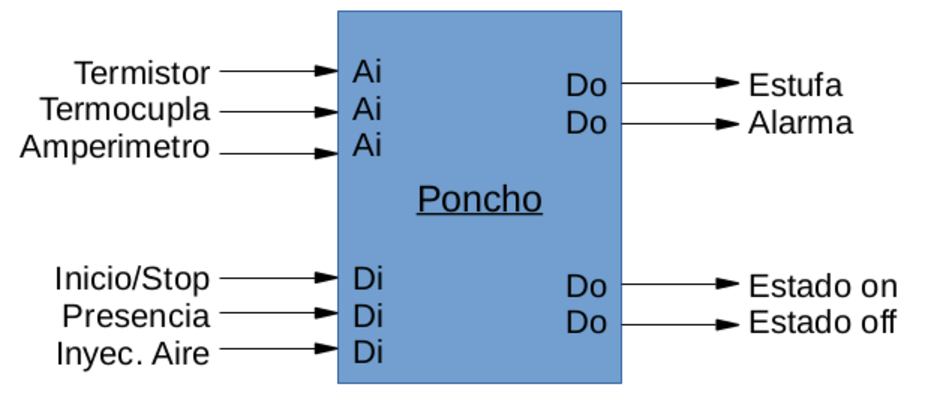
\includegraphics[width=.7\textwidth]{Figures/Cap_3/conexion_modo_1}
	\caption{Conexión en modo funcionamiento 1}
	\label{fig:conectPerifericos1}
\end{figure}

\begin{figure}[h!]
	\centering
	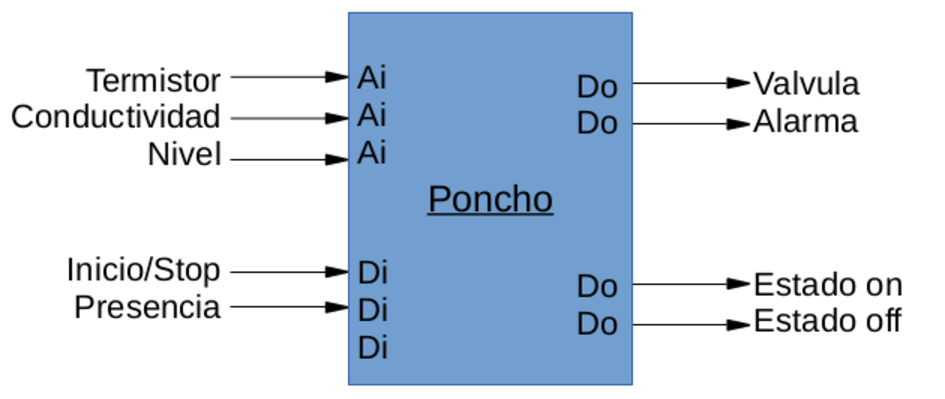
\includegraphics[width=.78\textwidth]{Figures/Cap_3/conexion_modo_2}
	\caption{Conexión en modo funcionamiento 2.}
	\label{fig:conectPerifericos2}
\end{figure}

Los puertos están preconfigurados y tienen asignaciones de pines predeterminadas, no obstante estos pueden modificarse desde la terminal al ingresar al modo de configuración.

En las figuras \ref{fig:renderPonchoTOP} y \ref{fig:renderPonchoBOT} se muestran las vistas del prototipo propuesto para desarrollar en el sistema piloto. 

\begin{figure}[h!]
	\centering
	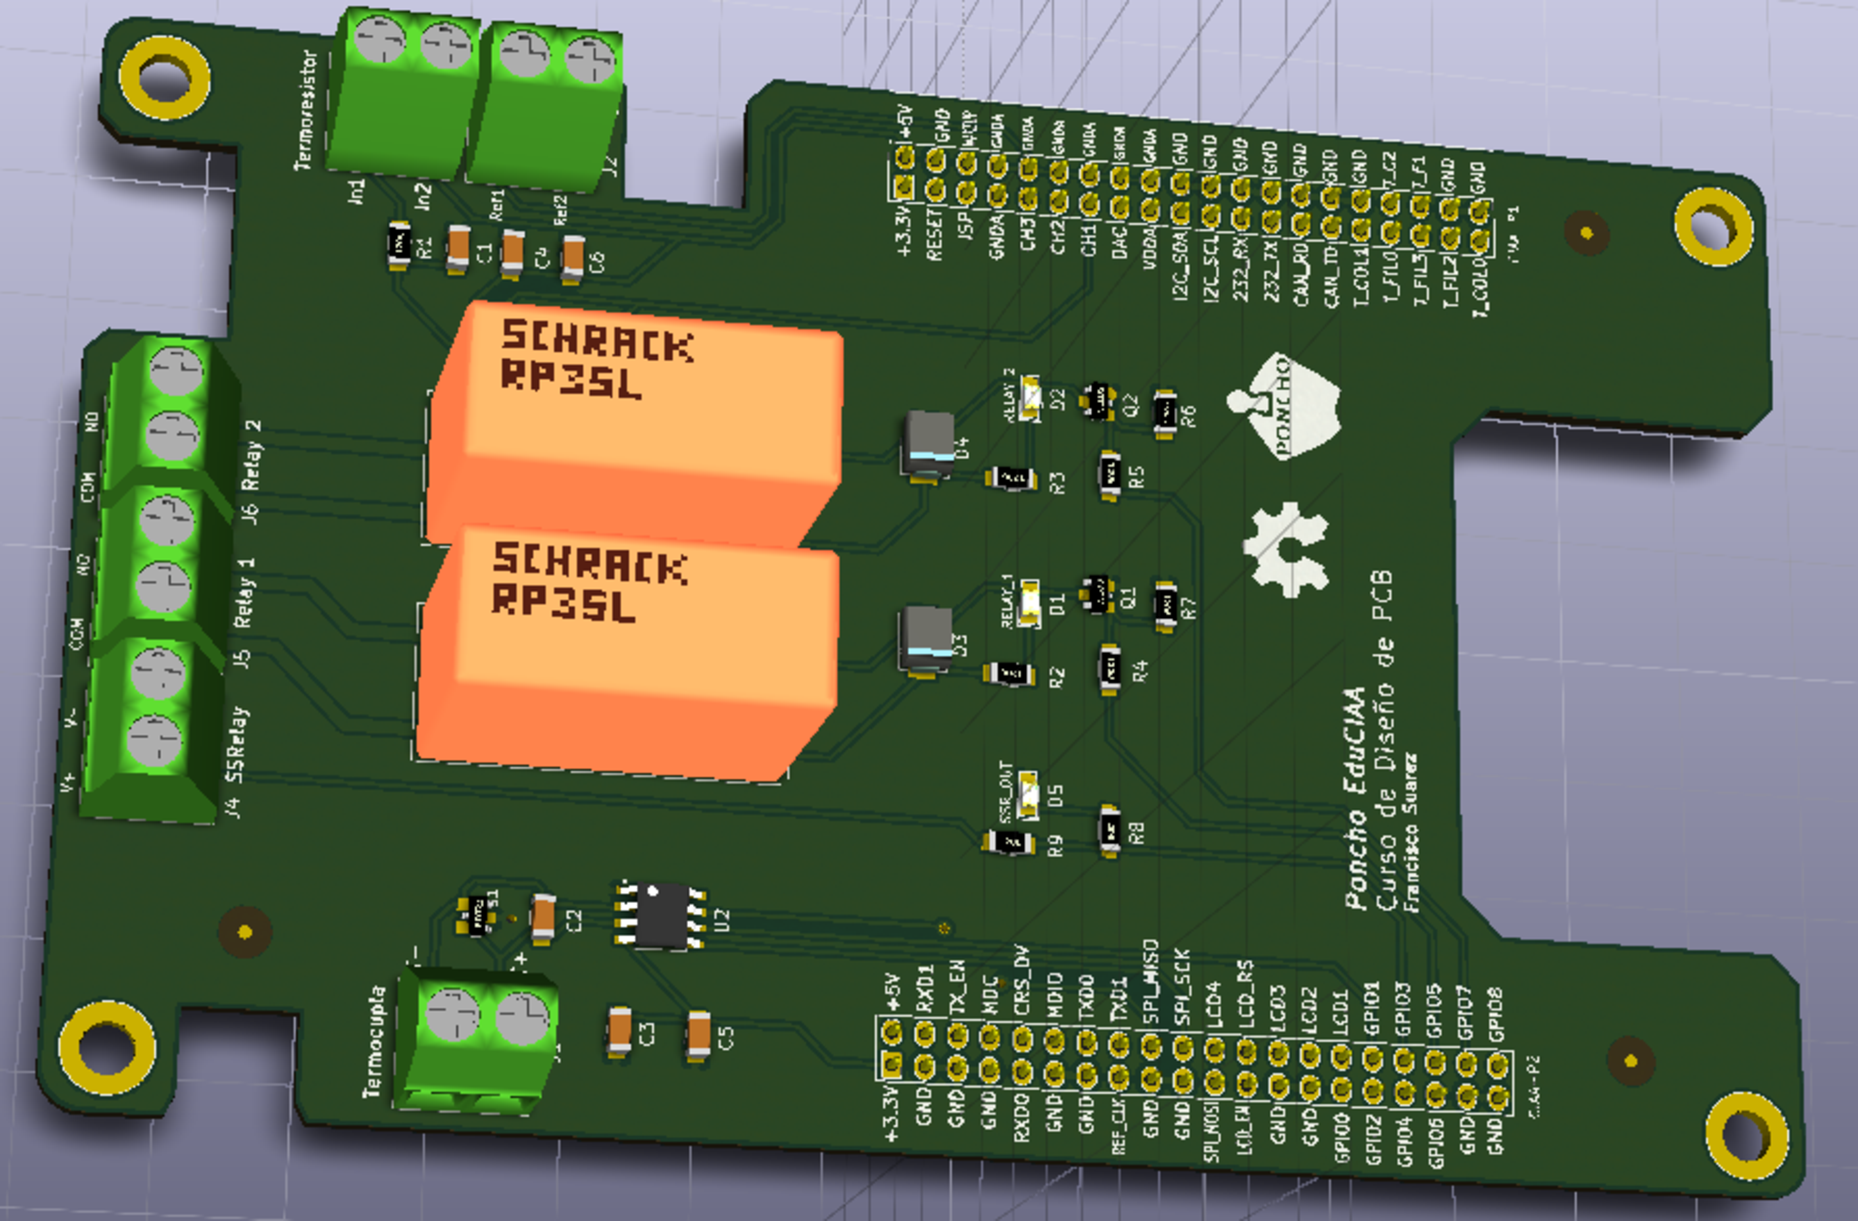
\includegraphics[width=.7\textwidth]{Figures/Cap_3/tempRelayPoncho_TOP}
	\caption{Render vista de arriba placa de interfaz.}
	\label{fig:renderPonchoTOP}
\end{figure}

\begin{figure}[h!]
	\centering
	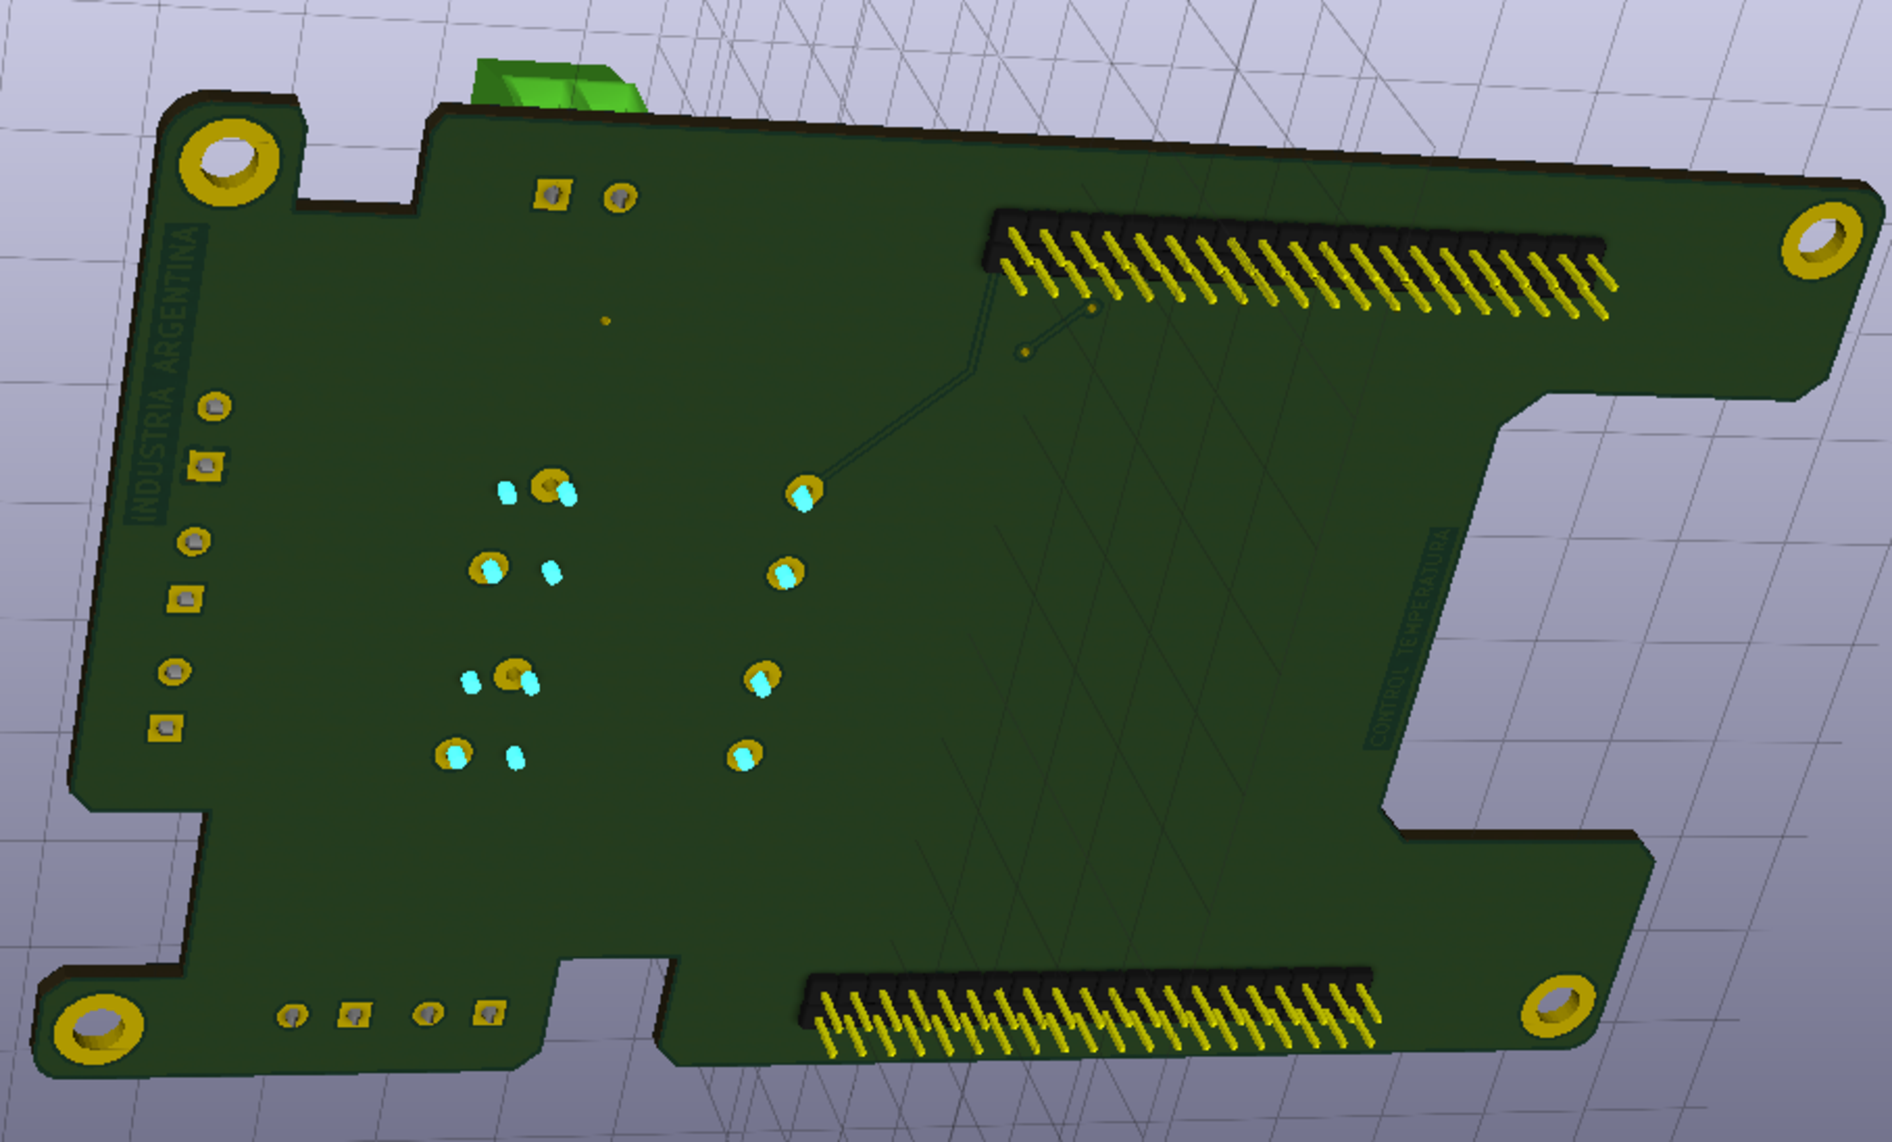
\includegraphics[width=.7\textwidth]{Figures/Cap_3/tempRelayPoncho_BOTTOM}
	\caption{Render vista de abajo de placa de interfaz.}
	\label{fig:renderPonchoBOT}
\end{figure}

La placa de la figura no llego a construirse hasta la fecha debido a que no se habían terminado de definir detalles relevantes respecto al numero y tipos de sensores y actuadores a utilizar.

En el Apéndice \ref{AppendixB} se encuentran los esquemáticos completos de las placa de expansión.
%----------------------------------------------------------------------------------------
%	SECTION 2
% La idea de esta sección es resaltar los problemas encontrados, los criterios utilizados y la justificación de las decisiones que se hayan tomado.
%----------------------------------------------------------------------------------------
\section{ Arquitectura del Software }

En función de los requerimientos vistos en \ref{subsec:Requerimientos} y de implementar los conocimientos aprendidos durante el posgrado, se determinaron los criterios para esta etapa.\\ 
En primer lugar se eligió usar lenguaje C y el sistema operativo FreeRTOS para la implementación.\
En segundo se diseñó el código de manera modularizado en tareas las cuales pueden funcionar de modo independiente según si la implementación lo requiere. \
En tercer lugar se tiene como modelo patrón el denominado \enquote{control ambiental} el cual se emplea cuando es un sistema con sensores que proporcionan información sobre el entorno y los actuadores pueden cambiar.\\

La aplicación cuenta los siguientes componentes:
\begin{itemize}
\item a. Interfaz de usuario (ingreso de parámetros, uart, lcd, alarmas).
\item b. Control de temperatura.
\item c. Monitoreo de nivel.
\item d. Monitoreo de conductividad.
\item e. Monitoreo de energía.
\item f. Control de tiempos.
\end{itemize}

Según el modo de funcionamiento seleccionado se tendrá una diferente configuración del software siempre dentro de la misma arquitectura y con pocas diferencias entre ellos. En la figura \ref{fig:diag_interfaces_m1} se muestran los diagramas de interfaces y procesos internos en el modo de funcionamiento 1. 
% AGREGAR UN DIAGRAMA DE INTERACCION ENTRE COMPONENTES ¿? ******************************
\begin{figure}[h!]
	\centering
	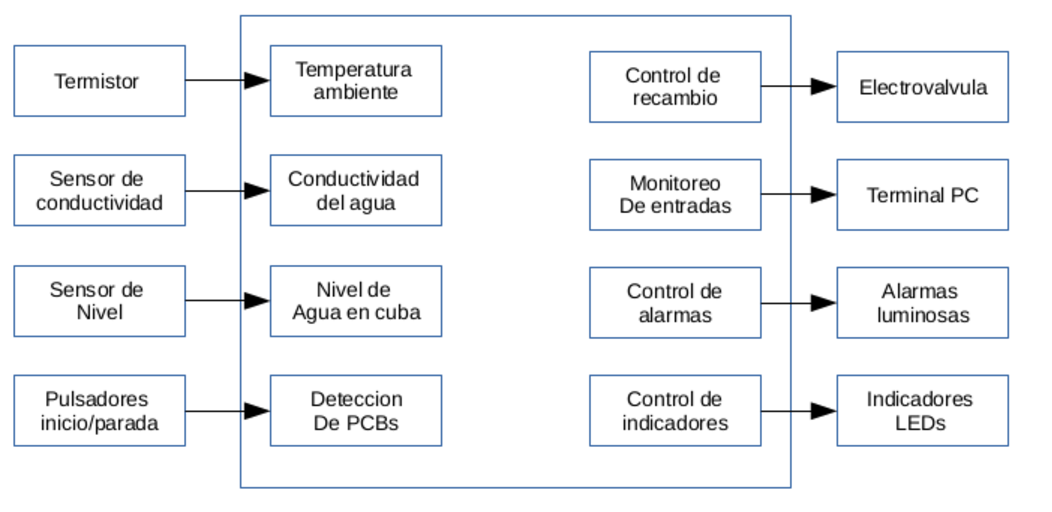
\includegraphics[width=1.0\textwidth]{Figures/Cap_3/diagrama_interfaces_1}
	\caption{ Vinculación de las periféricos del sistema con las interfaces internas en el modo 1. }
	\label{fig:diag_interfaces_m1}
\end{figure}
 
En la figura \ref{fig:diag_comunicacion_m1} se muestra el diagrama de comunicación entre los procesos originados para el caso de funcionamiento 1. Se nota su relación con los componentes de la aplicación: a,b,e y f.

\begin{figure}[h!]
	\centering
	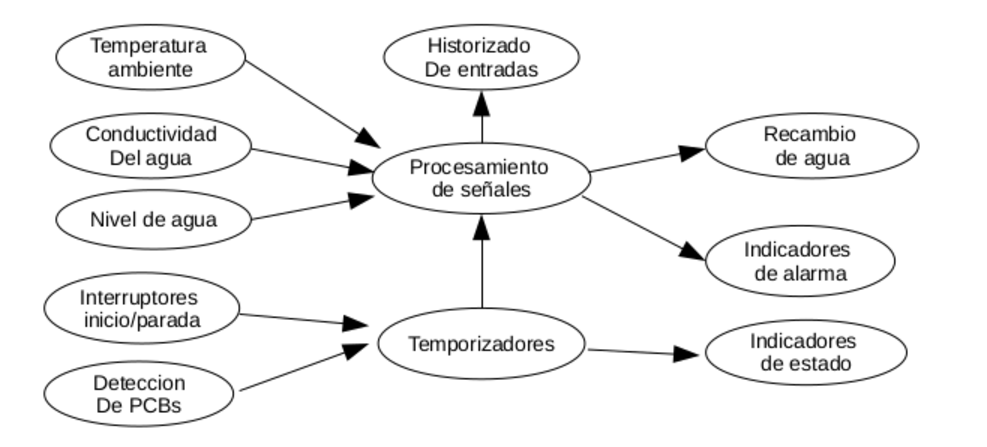
\includegraphics[width=1.0\textwidth]{Figures/Cap_3/diagrama_comunicacion_1}
	\caption{ Diagrama de comunicación entre procesos en el modo 1. }
	\label{fig:diag_comunicacion_m1}
\end{figure}
 
En la figura \ref{fig:diag_interfaces_m2} se muestran los diagramas de interfaces y procesos internos en el modo de funcionamiento 2.  Se nota que hay poca diferencia con el caso anterior, solo tienen activos otros procesos de interfaz.

\begin{figure}[h!]
	\centering
	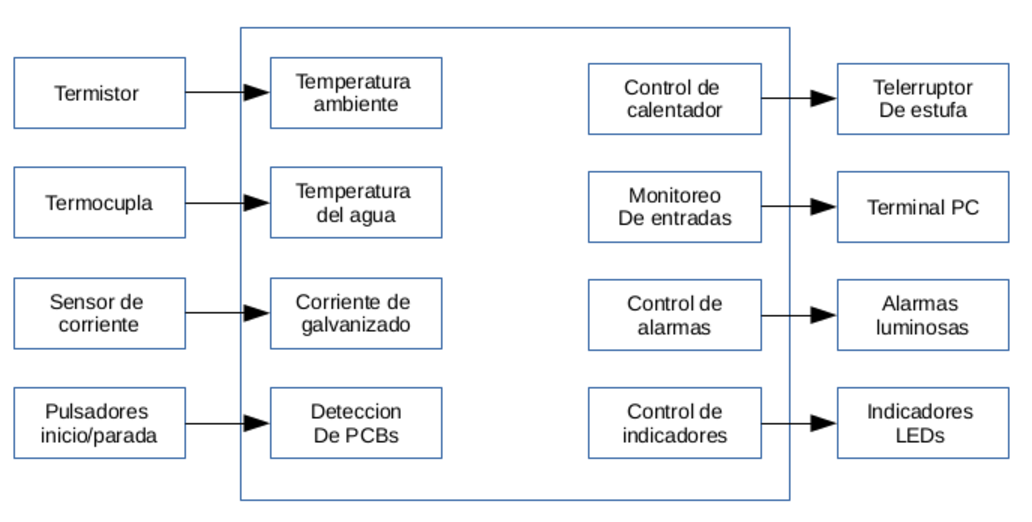
\includegraphics[width=1.0\textwidth]{Figures/Cap_3/diagrama_interfaces_2}
	\caption{ Vinculación de las periféricos del sistema con las interfaces internas en el modo 2.}
	\label{fig:diag_interfaces_m2}
\end{figure}

En la figura \ref{fig:diag_comunicacion_m2} se muestra el diagrama de comunicación entre los procesos originados para el caso de funcionamiento 2. Se nota su relación con los componentes de la aplicación: a,b,c, y f.

\begin{figure}[h!]
	\centering
	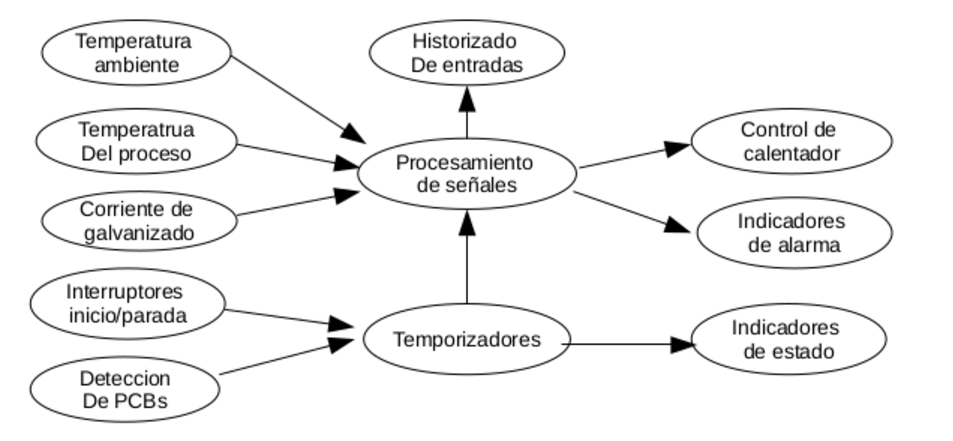
\includegraphics[width=1.0\textwidth]{Figures/Cap_3/diagrama_comunicacion_2}
	\caption{ Diagrama de comunicación entre procesos en el modo 2. }
	\label{fig:diag_comunicacion_m2}
\end{figure}
 
\subsection{ Capas de abstracción }

el sistema se divide en capas que otorgan abstracción del hardware y además permiten obtener código mas reutilizable e independiente de la plataforma. Estos son cambios que el cliente puede solicitar a futuro.
En la figura \ref{fig:diagrama_capas} se observa el patrón de capas de la arquitectura.

% Agregar una imagen con la division en capas del firmware.
\begin{figure}[h!]
	\centering
	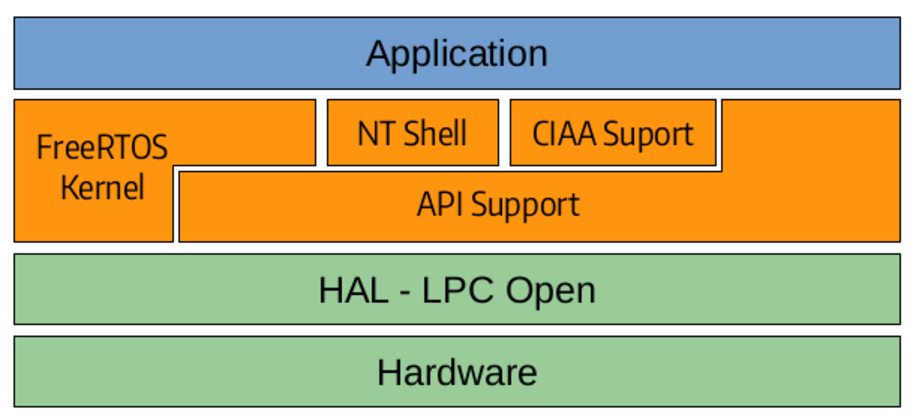
\includegraphics[width=.8\textwidth]{Figures/Cap_3/diagrama_capas}
	\caption{Estructuras de capas del sistema.}
	\label{fig:diagrama_capas}
\end{figure}
 
Las capas son las siguientes: 
\begin{itemize}
\item \emph{Aplicación:} Rutinas creadas para cada una de las tareas.
\item \emph{NT Shel:} Implementa el interprete de comandos ingresados externamente e internamente, a fin de configurar o de obtener información del dispositivo \citep{nt_shell}.
\item \emph{FreeRTOS:} Sistema operativo, controla la comunicación entre tareas, acceso a recursos compartidos y el scheduler. \cite{free_rtos}.
\item \emph{API Support:} implementa las rutinas de acceso y configuración de los distintos periféricos.
\item \emph{HAL:} rutinas de acceso al hardware, implementada con la librería LPC OPEN para el uP LPC43XX \citep{lpcopen}.
\end{itemize}


\subsection{ Diseño }

Por la necesidad de dividir el problema en partes menores para hacerlo mas escalable, mantenible y debugueable, el sistema se divide en subsistemas o tareas cooperativas entre si. Las mismas están definidas como:
\begin{itemize}
	\item Monitoreo de entradas analógicas-digitales.
	\item Control de salidas digitales.
	\item Manejo de terminal y comandos.
	\item Manejo de memoria y log de datos.
\end{itemize}

En la figura \ref{fig:diag_Tareas} muestra un diagrama de estado general de las tareas y la interacción entre ellas.
% Diagrama de tareas y conexion entre ellas
\begin{figure}[h!]
	\hspace{-1.0cm}
%	\centering
	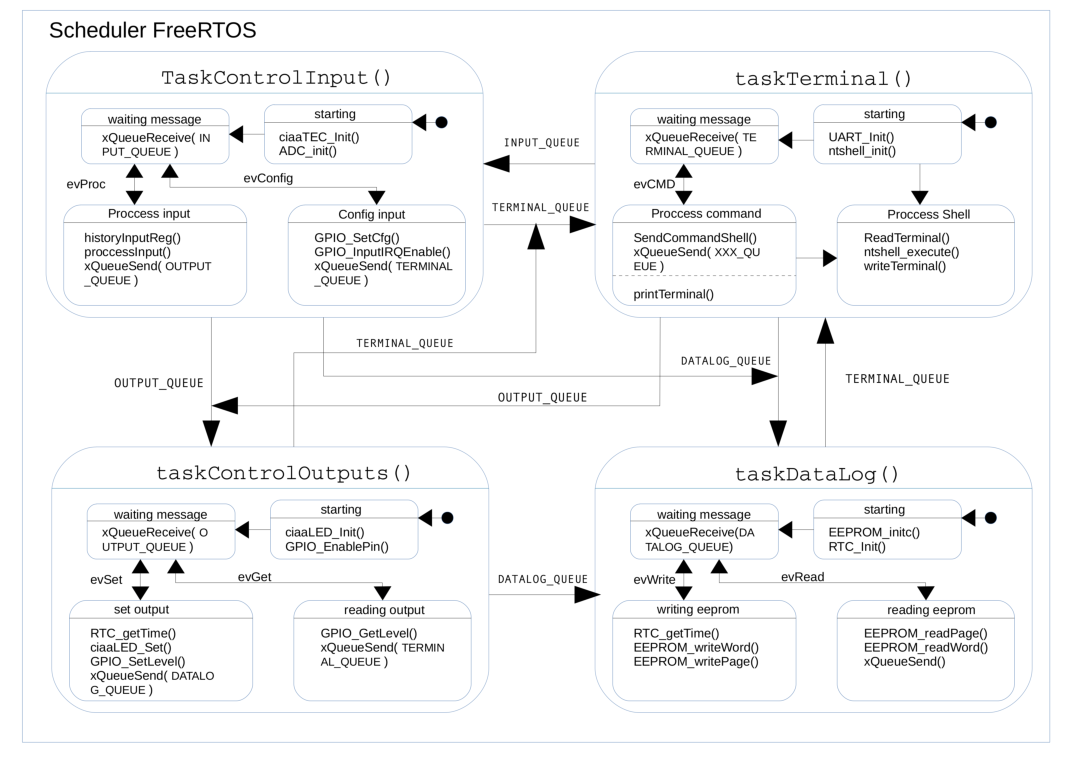
\includegraphics[width=1.1\textwidth]{Figures/Cap_3/diagrama_tareas}
	\caption{ Interacción entre tareas. }
	\label{fig:diag_Tareas}
\end{figure}

\section{ Sistemas control de entradas }
El monitoreo de las entradas se divide en subestados según la opción de funcionamiento elegida, y a la vez se puede encontrar en funcionamiento normal, en estado falla o en reconfiguración. 
La lectura de las entradas digitales las hace por interrupción mientras que las analógicas las hace por polling según tiempos por default a través del terminal. La figura \ref{fig:diag_TareasInp} muestra el diagrama de estados de la tarea.
 
% Se puede pensar tambien en poder poner la tarea en suspension hasta no tener una habilitacion por algun semaforo o por alguna tarea que la suspenda, tendria que ser si o si la taskTerminal. O bien por algun estado de error que la deje esperando la normalizacion. 
\begin{figure}[h!]
	\hspace{-0.5cm}
%	\centering
	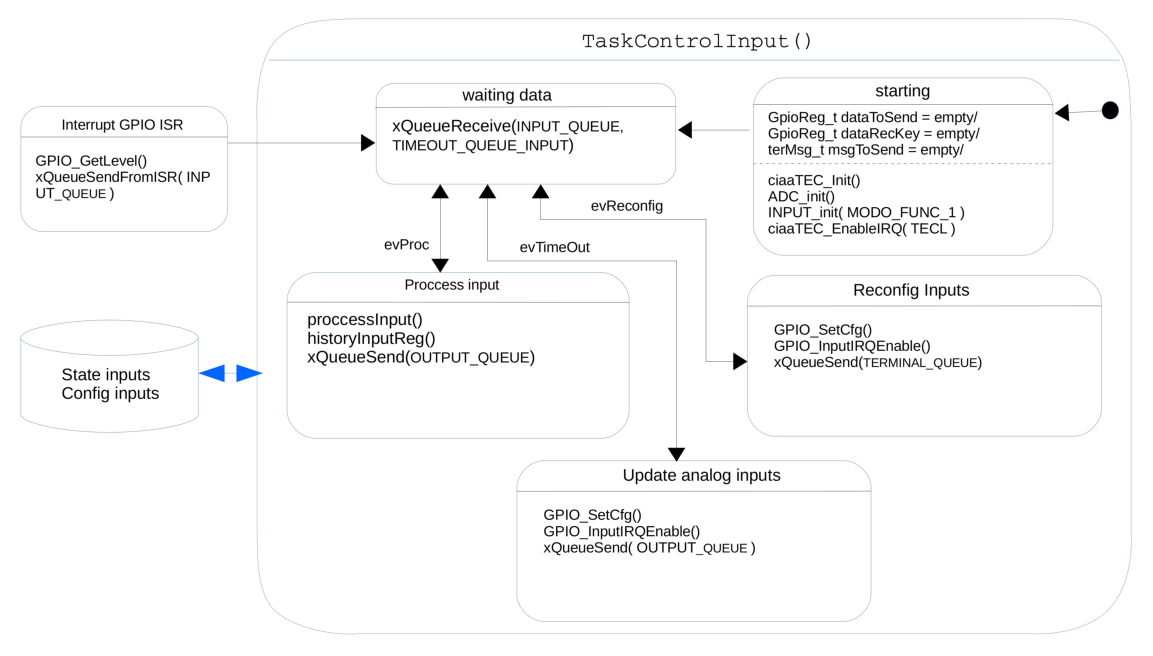
\includegraphics[width=1.05\textwidth]{Figures/Cap_3/diagrama_tarea_input}
	\caption{ Diagrama de estados de la tarea control de entradas. }
	\label{fig:diag_TareasInp}
\end{figure}

Se observa que a medida que se actualizan los valores de las registros de las entradas, la tarea ejecuta acciones vinculadas con cada una de ellas. Luego en función de estas acciones evalúa si debe enviar un mensaje hacia otra de las tareas, siempre y cuando la tarea destino esté habilitada y en modo activo.
El manejo de los temporizadores de duración de cada etapa es implementado por esta tarea, ya que es dependiente del estado de entradas digitales.   

\section{ Sistemas control de salidas }
El control de las salidas esta ligado expresamente a las acciones externas. Las acciones llegan por cambios ocurridos en las entradas o pueden ser forzar a través del terminal de PC. Por esta razón éste modulo no es pausado en ningún momento del funcionamiento.\\
Las acciones que activan las salidas están parametrizadas en un registro interno del módulo. Cuando la tarea verifica que se debe ejecutar un cambio en una salida entonces verifica también si debe reenviar algún parámetro hacia otra tarea.
La figura \ref{fig:diag_TareasOut} muestra el diagrama de estados de la tarea.
 
\begin{figure}[h!]
	\hspace{-0.5cm}
	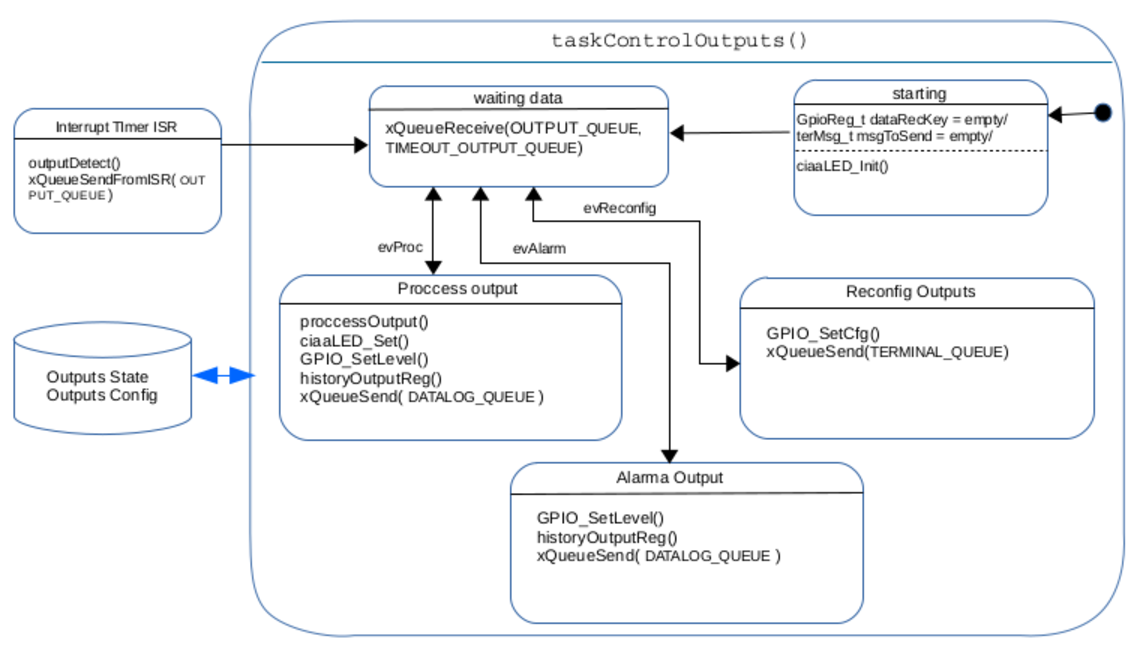
\includegraphics[width=1.0\textwidth]{Figures/Cap_3/diagrama_tarea_output}
	\caption{ Diagrama de estados de la tarea control de salidas. }
	\label{fig:diag_TareasOut}
\end{figure}

\section{ Sistemas control de terminal-Shell }
Este modulo se encarga de emular la terminar con la PC procesando comandos y consultas. Esta tarea es opcional para el sistema pero es importante para obtener información de históricos y realizar test de los puertos del hardware. 
%---- VER si queda este parrafo.
Originariamente se pensó también que la misma ajustaría los parámetros de alarma y de tiempos por etapa a partir del ingreso de información del lote a procesar. Luego como se determino que el sistema fueran modular este concepto no es aplicable. No obstante se pueden ajustar parámetros de tiempos y de niveles de alarma.

La figura \ref{fig:diag_TareasShell} muestra el diagrama de estados de la tarea.
% Colocar diagrama de estados
\begin{figure}[h!]
	\hspace{-0.1cm}
	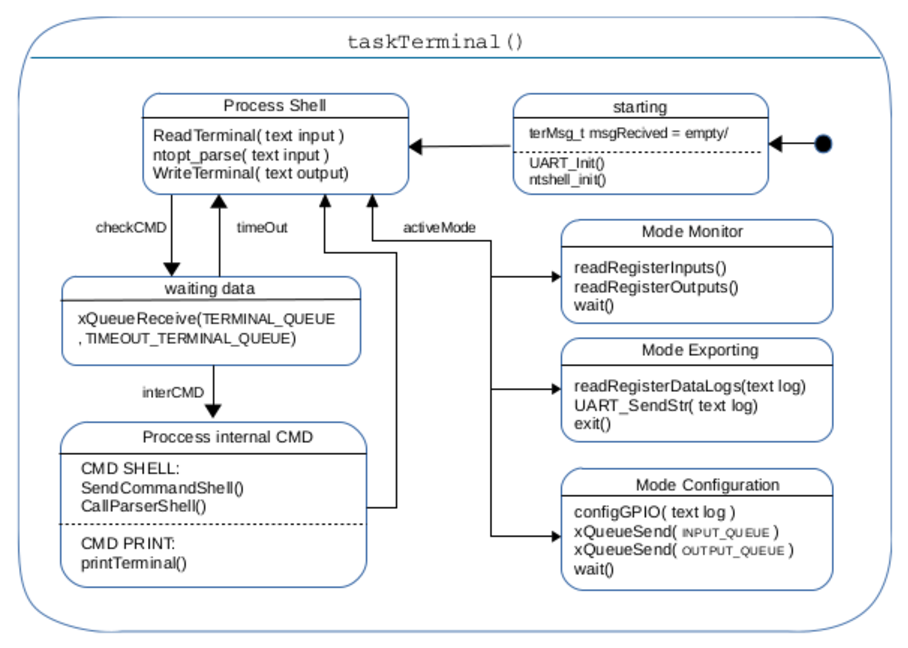
\includegraphics[width=1.0\textwidth]{Figures/Cap_3/diagrama_tarea_terminal}
	\caption{ Diagrama de estados de la tarea terminal de comunicación. }
	\label{fig:diag_TareasShell}
\end{figure}

Los estados están predeterminados por los comandos implementados de los cuales se puede agregar hasta 255. En la tabla \ref{tablas_comandos} se resumen los comandos implementados.

\begin{table}[]
\hspace{-1.5cm}
\begin{flushleft}
\begin{tabular}{|m{1.8cm}|m{3cm}|m{4.5cm}|m{4.5cm}|}\hline
{\textbf{Comando}} & {\textbf{Función}} & {\textbf{Descripción}} & {\textbf{Parámetros}} \\ \hline
{\textit{hist}} & {Registros históricos} & { Devuelve una lista con los últimos registros guardados en memoria.} & {Ninguno} \\ \hline
{\textit{mon}} & {Monitoreo de puertos} & {Muestra el valor y la variación de las entradas y salidas del dispositivo.} & {Ninguno.} \\ \hline
{\textit{conf}} & {Configuración de parámetros} & {Configura valores máximo, mínimo y tiempos de muestreo de un pin.} & {nXmax, nXmin, tXmax, tXmin. X: Número de parámetro. n: Nivel. t: Tiempo.} \\ \hline
{\textit{test}} & {Testing de puertos} & {Modifica el valor de una entrada para evaluar el comportamiento del sistema.} & {PX val, donde P=I/O, X=id puerto, val= valor del puerto..} \\ \hline
{\textit{time}} & {Configura el calendario} & {Modificar la hora y fecha del calendario interno usado en la grabación de históricos.} & {c DDMMAA, calendario día(DD), mes(MM), año(AA).t HHMMSS, tiempo hora(HH), minutos(MM), segundos(SS).} \\ \hline
\end{tabular}
\end{flushleft}
\caption{Descripción tablas de comandos.}
\label{tablas_comandos}
\end{table}


\section{ Sistemas gestión de datos }

Se encarga de manejar los registros que deben ser guardados y leídos de la memoria EEPROM interna. Los datos a ser grabados son leídos de espacios de memoria RAM compartidos y los datos leídos son almacenados en un buffer compartido de la tarea para luego ser enviados a la tarea solicitante.
% Colocar diagrama de estados
La figura \ref{fig:diag_TareasLogs} muestra el diagrama de estados de la tarea.

\begin{figure}[]
	\hspace{-1.5cm}
	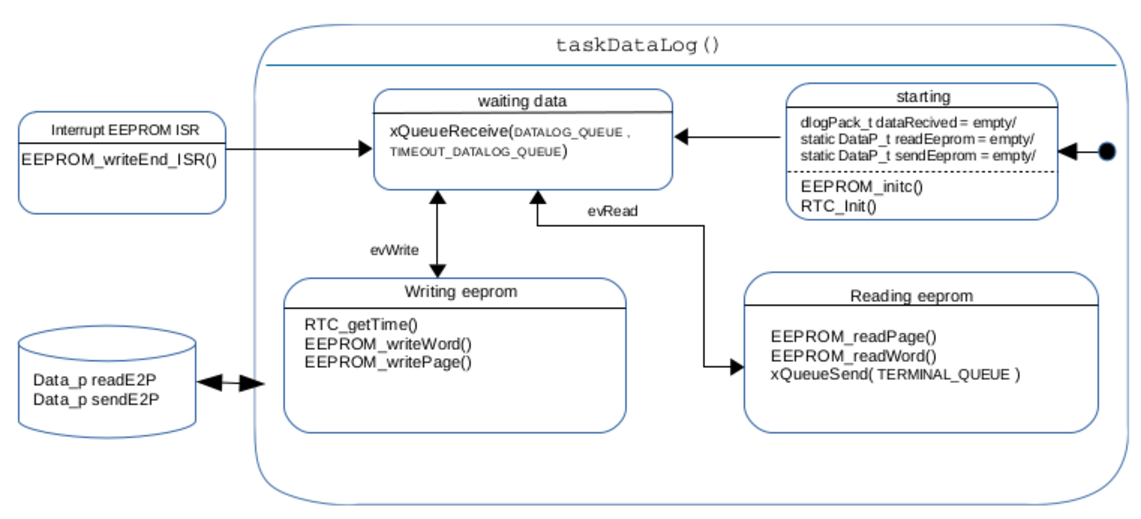
\includegraphics[width=1.2\textwidth]{Figures/Cap_3/diagrama_tarea_datalog}
	\caption{Diagrama de estados de la tarea manejo de datos en memoria.}
	\label{fig:diag_TareasLogs}
\end{figure}






%% Chapter Template

\chapter{Ensayos y Resultados} % Main chapter title

\label{Chapter4} % Change X to a consecutive number; for referencing this chapter elsewhere, use \ref{ChapterX}

%----------------------------------------------------------------------------------------
%	SECTION 1
%----------------------------------------------------------------------------------------

\section{Pruebas funcionales del hardware}
\label{sec:pruebasHW}

La idea de esta sección es explicar cómo se hicieron los ensayos, qué resultados se obtuvieron y analizarlos.
 
%% Chapter Template

\chapter{Conclusiones} % Main chapter title

\label{Chapter5} % Change X to a consecutive number; for referencing this chapter elsewhere, use \ref{ChapterX}


%----------------------------------------------------------------------------------------

%----------------------------------------------------------------------------------------
%	SECTION 1
%----------------------------------------------------------------------------------------

\section{Conclusiones generales }

La idea de esta sección es resaltar cuáles son los principales aportes del trabajo realizado y cómo se podría continuar. Debe ser especialmente breve y concisa. Es buena idea usar un listado para enumerar los logros obtenidos.

%----------------------------------------------------------------------------------------
%	SECTION 2
%----------------------------------------------------------------------------------------
\section{Próximos pasos}

Acá se indica cómo se podría continuar el trabajo más adelante.
 

%----------------------------------------------------------------------------------------
%	CONTENIDO DE LA MEMORIA  - APÉNDICES
%----------------------------------------------------------------------------------------

\appendix % indicativo para indicarle a LaTeX los siguientes "capítulos" son apéndices

% Incluir los apéndices de la memoria como archivos separadas desde la carpeta Appendices
% Descomentar las líneas a medida que se escriben los apéndices

% Appendix A

\chapter{Casos de Uso} % Main appendix title

\label{AppendixA} % For referencing this appendix elsewhere, use \ref{AppendixA}

Referencias:

Ref 1-  Disparadores:  Evento comienza el caso de uso.\\
Ref 2 - Flujo básico:  Pasos del escenario, desde que es disparado hasta que alcanza su objetivo.\\
Ref 3 - Flujo alternativo:  Pasos alternativos al flujo básico. \\
Ref 4-  Pre-Condiciones:  Condiciones que deben estar presentes para que se pueda iniciar el caso de uso.\\
Ref 5-  Pos-Condiciones: Condiciones que deben estar presentes para que se pueda finalizar el caso de uso.\\
Ref 6-  Modo 1: Medición de conductividad, nivel y control de temperatura.\\
Ref 7-  Modo 2: Medición de corriente, tensión, nivel y control de temperatura.\\

% Tablas con los casos de Uso --------------------------------------------------------------------%
% Puesta en alta del dispositivo:
\begin{table}[ht]
\begin{flushleft}
\begin{tabular}{|m{3.2cm}|m{11cm}|}\hline
\multicolumn{1}{|c|}{\textbf{Título}} & \multicolumn{1}{c|}{\textbf{Descripción}} \\ \hline
{1. Nombre} & {Puesta en alta del dispositivo.} \\ \hline
1.1. Descripción  & Secuencia de instalación de dispositivo en las cubas de control. \\ \hline
1.2. Actor principal  & Técnico instalador. \\ \hline
1.3. Disparadores  & Alimentación de la unidad. \\ \hline
2. Flujo de eventos &  \\ \hline
\multicolumn{1}{|l|}{2.1. Flujo básico} & {2.1.1. El sistema inicia el ciclo de encendido y se prepara para evaluar los rangos de las entradas de una por vez. 2.1.4  Censa que los  de los termostatos sean los correctos. (a definir)} \\ \cline{ 2- 2}
\multicolumn{1}{|l|}{} & 2.1.2. Para cada uno emite una señal a definir en caso de ser correcto y otra en caso de ser incorrecto.  \\ \cline{ 2- 2}
\multicolumn{1}{|l|}{} & 2.1.3. Censa que los valores de corriente sobre los lazos de control de conductividad sean los correctos, según el máximo y el mínimo admisible.(a definir)  \\ \cline{ 2- 2}
\multicolumn{1}{|l|}{} & 2.1.4. Censa que los valores de los termostatos sean los correctos. (a definir) \\ \cline{ 2- 2}
\multicolumn{1}{|l|}{} & 2.1.5. Censa los valores de las entrada de nivel, que deben estar dentro de los establecidos según RINB242? \\ \hline
2.2. Flujo alternativo  & 2.1.6. Si alguno de los sensores no esta dentro de los valores se bloquea el proceso hasta que se seleccione ignorar o se normalice el parámetro.  \\ \hline
3. Requerimientos especiales & Botón de encendido liberado. Selector de modo de funcionamiento en posición. \\ \hline
4. Pre Condiciones  & Interfaces de sensores conectados.  \\ \hline
5. Pos Condiciones & El dispositivo queda en modo espera a la señal de inicio de ciclo, midiendo según los requerimientos RFTEM112,121,131,153? y mostrándolos por uart los valores de cada uno. \\ \hline
\end{tabular}
\end{flushleft}
\caption{Descripción caso de uso puesta en alta}
\label{caso_uso_alta}
\end{table}

% Secuencia de pasos para configurar dispositivo en el modo 1 de uso:
\begin{table}[h!]
\begin{flushleft}
\begin{tabular}{|m{3cm}|m{11cm}|}\hline
\multicolumn{1}{|c|}{\textbf{Título}} & \multicolumn{1}{c|}{\textbf{Descripción}} \\ \hline
1. Nombre & Puesta en funcionamiento en Modo 1 \\ \hline
1.1 Breve descripción  & Secuencia de control de un ciclo completo dentro de las cuba controlada  \\ \hline
1.2 Actor principal  & Operario (Op) \\ \hline
1.3 Disparadores  & Pulsación de botón inicio \\ \hline
2. Flujo de eventos &  \\ \hline
\multicolumn{ 1}{|l|}{2.1. Flujo básico} & 2.1.1. El sistema detecta la presencia de las placas con el detector colocado en la cuba. \\ \cline{ 2- 2}
\multicolumn{ 1}{|l|}{} & 2.1.2. El sistema inicia el conteo del tiempo preestablecido para esa etapa utilizando un indicar luminoso para indicar al Op. \\ \cline{ 2- 2}
\multicolumn{ 1}{|l|}{} & 2.1.3. El sistema continua controlando los parámetros de temperatura y nivel durante todo el ciclo y transmitiendo los valores por uart. \\ \cline{ 2- 2}
\multicolumn{ 1}{|l|}{} & 2.1.4. Completado el ciclo el sistema emite una señal al Op para que se disponga a retirar las placas de la cuba. \\ \hline
\multicolumn{ 1}{|l|}{2.2. Flujo alternativo } & 2.2.1. El sistema no detecta la placa con los sensores de presencia y no inicia el conteo de tiempo. \\ \cline{ 2- 2}
\multicolumn{ 1}{|l|}{} & 2.2.2. Si se colocan las placas o se anula la entrada del sensor el proceso vuelve a 2.1.2 del flujo básico. \\ \hline
\multicolumn{ 1}{|l|}{2.3. Flujo alternativo } & 2.3.1. El Op retira las placas de la cuba antes de completado el tiempo reglamentario. El sistema emite una seña de alarma para que se restablezca la placa durante 15 segundos. \\ \cline{ 2- 2}
\multicolumn{ 1}{|l|}{} & 2.3.2. Si se restablece la placa antes de cumplirse los 15 segundos se retorna al paso normal en el que se encontraba. Sino vuelve el contador de tiempo a cero y deja un indicador de alarma encendido hasta que se lo anule manualmente y vuelve al punto 2.1.5 del flujo básico. \\ \hline
\multicolumn{ 1}{|l|}{2.4. Flujo alternativo } & 2.4.1. El sistema detecta que la temperatura o el nivel fuera de valor nominal por mas de 5 minutos emite una alarma y continua el proceso normal hasta 2.1.5.\\ \cline{ 2- 2}
\multicolumn{ 1}{|l|}{} & 2.4.2.  Finalizado el tiempo no permite iniciar un nuevo ciclo hasta que las parámetros de control vuelvan a sus valores nominales.  \\ \hline
3. Requerimientos especiales & El sistema debe estar configurado en el Modo 1. \\ \hline
4. Pre condiciones  &  Sistema energizado e inicializado.   \\ \hline
5. Pos condiciones &  Queda en modo espera controlando los parámetros según los requerimientos RFTEM112,121,131,153? \\ \hline
\end{tabular}
\end{flushleft}
\caption{Descripción caso de uso en Modo 1}
\label{caso_uso_func_1}
\end{table}

% Secuencia de pasos para configurar dispositivo en el modo 2 de uso:

\begin{table}[h!]
\begin{flushleft}
\begin{tabular}{|m{3cm}|m{11cm}|}
\hline
\multicolumn{1}{|c|}{\textbf{Título}} & \multicolumn{1}{c|}{\textbf{Descripción}} \\ \hline
1. Nombre & Puesta en funcionamiento en Modo 2. \\ \hline
1.1 Breve descripción  & Secuencia de control de un ciclo completo dentro de las cuba controlada. \\ \hline
1.2 Actor principal  & Operario (Op) \\ \hline
1.3 Disparadores  & Pulsación de botón inicio. \\ \hline
2. Flujo de eventos &  \\ \hline
\multicolumn{ 1}{|l|}{2.1 Flujo básico} & 2.1.1. El sistema detecta la presencia de las placas con el detector colocado en la cuba.2.1.2  El sistema detecta la  umbral y comienza a integrar el valor hasta llegar al total necesario.2.1.4  Completado el ciclo el sistema emite una señal al Op para que se disponga a retirar las placas de la cuba. \\ \cline{ 2- 2}
\multicolumn{ 1}{|l|}{} & 2.1.2. El sistema detecta la corriente umbral y comienza a integrar el valor hasta llegar al total necesario. \\ \cline{ 2- 2}
\multicolumn{ 1}{|l|}{} & 2.1.3. El sistema inicia un indicar luminoso para indicar al Op que la etapa esta en proceso. \\ \hline
\multicolumn{ 1}{|l|}{2.2. Flujo alternativo} & 2.2.1. El valor de temperatura se va de rango por mas de 10 minutos, el sistema emite una alarma sin interrumpir el proceso. \\ \hline
\multicolumn{ 1}{|l|}{2.3. Flujo alternativo} & 2.3.1. Si se retiran las placas de la cuba antes de que el procesos finalice, o el valor de corriente cae debajo de un valor mínimo aceptable por mas de 1 minuto se considera una situación anormal y se emite una alarma.  \\ \cline{ 2- 2}
\multicolumn{ 1}{|l|}{} & 
2.3.2. Si no se restablece el parámetro por mas de 30 segundos los contadores se vuelven a cero y se deja una alarma encendida, sino retorna al proceso al momento en que fue interrumpido. \\ \hline
3. Requerimiento especial & El sistema debe estar configurado en el Modo 2.\\ \hline
4. Pre condiciones  & Sistema energizado e inicializado.  \\ \hline
5. Pos condiciones & Queda en modo espera controlando los parámetros según los requerimientos RFTEM112,121,131,153? \\ \hline
\end{tabular}
\end{flushleft}
\caption{Descripción caso de uso en Modo 2}
\label{caso_uso_func_2}
\end{table}



% Appendix A

\chapter{Esquemáticos} % Main appendix title
\label{AppendixB} % For referencing this appendix elsewhere, use \ref{AppendixA}

\begin{sidewaysfigure}[!ht]
	\centering
	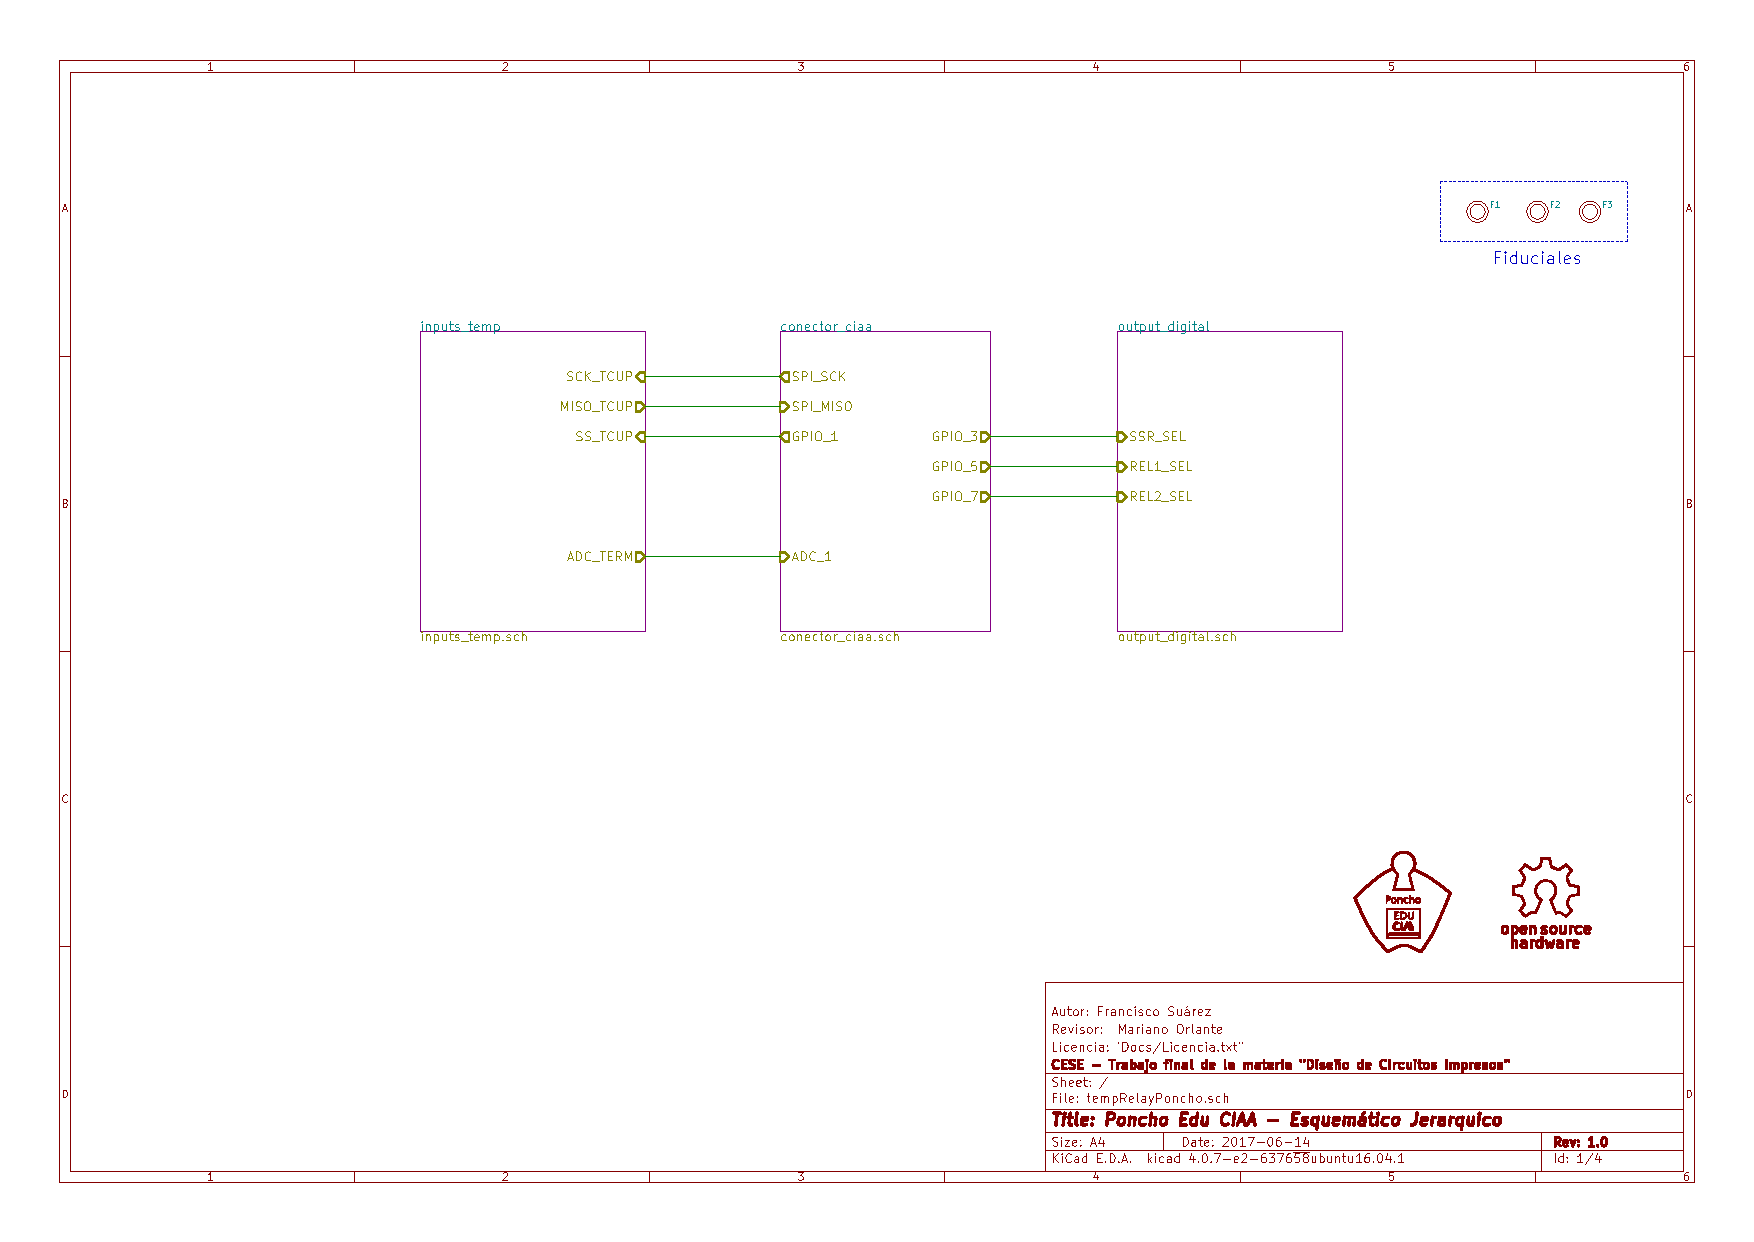
\includegraphics[width=0.9\textwidth]{Figures/Appendices/sch_mainPoncho}
	\caption{Esquemático jerárquico del poncho EduCiaa.}
	\label{fig:schMainPoncho}
\end{sidewaysfigure}


\begin{sidewaysfigure}[h!]
	\centering
	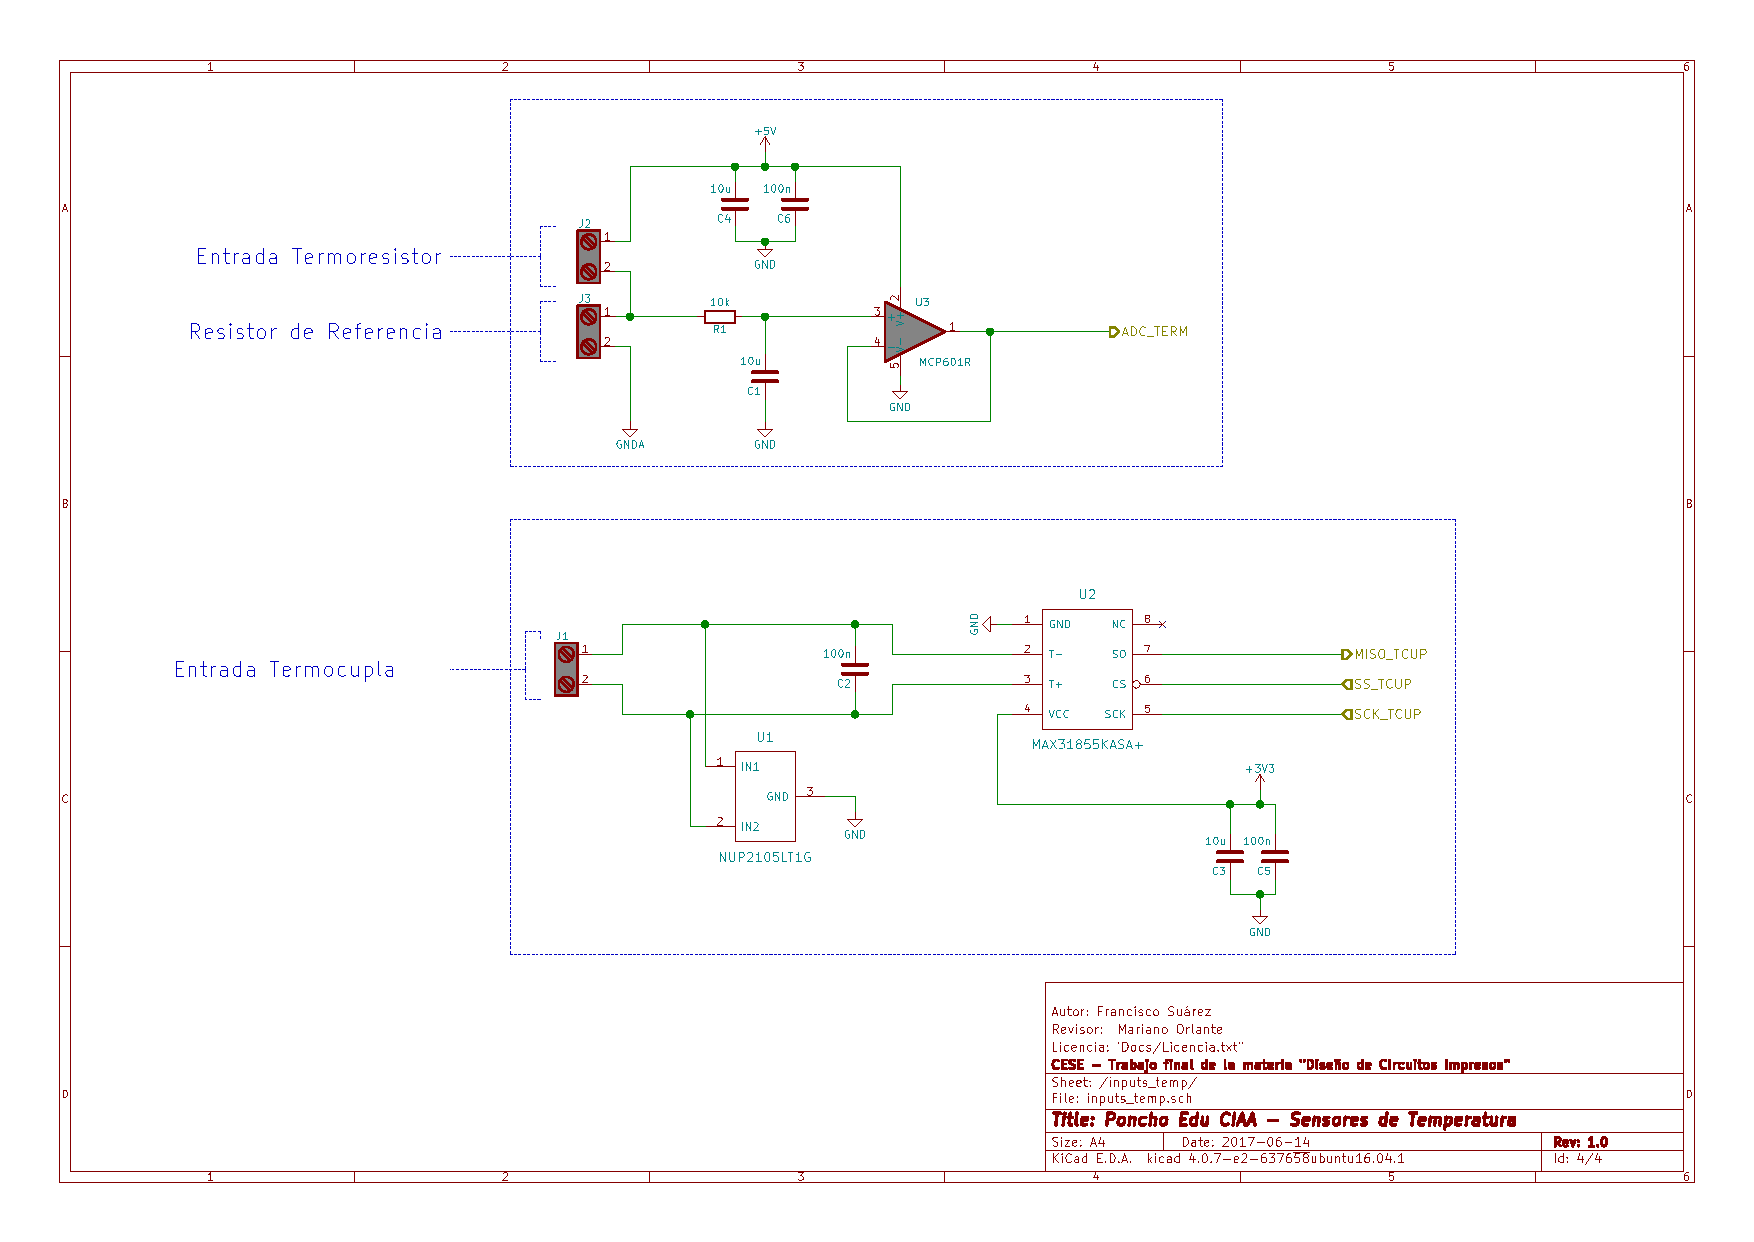
\includegraphics[width=1\textwidth]{Figures/Appendices/sch_inpTempTerm}
	\caption{Esquemático entradas de termocupla y termistor.}
	\label{fig:schEntradas}
\end{sidewaysfigure}


\begin{sidewaysfigure}[h!]
	\centering
	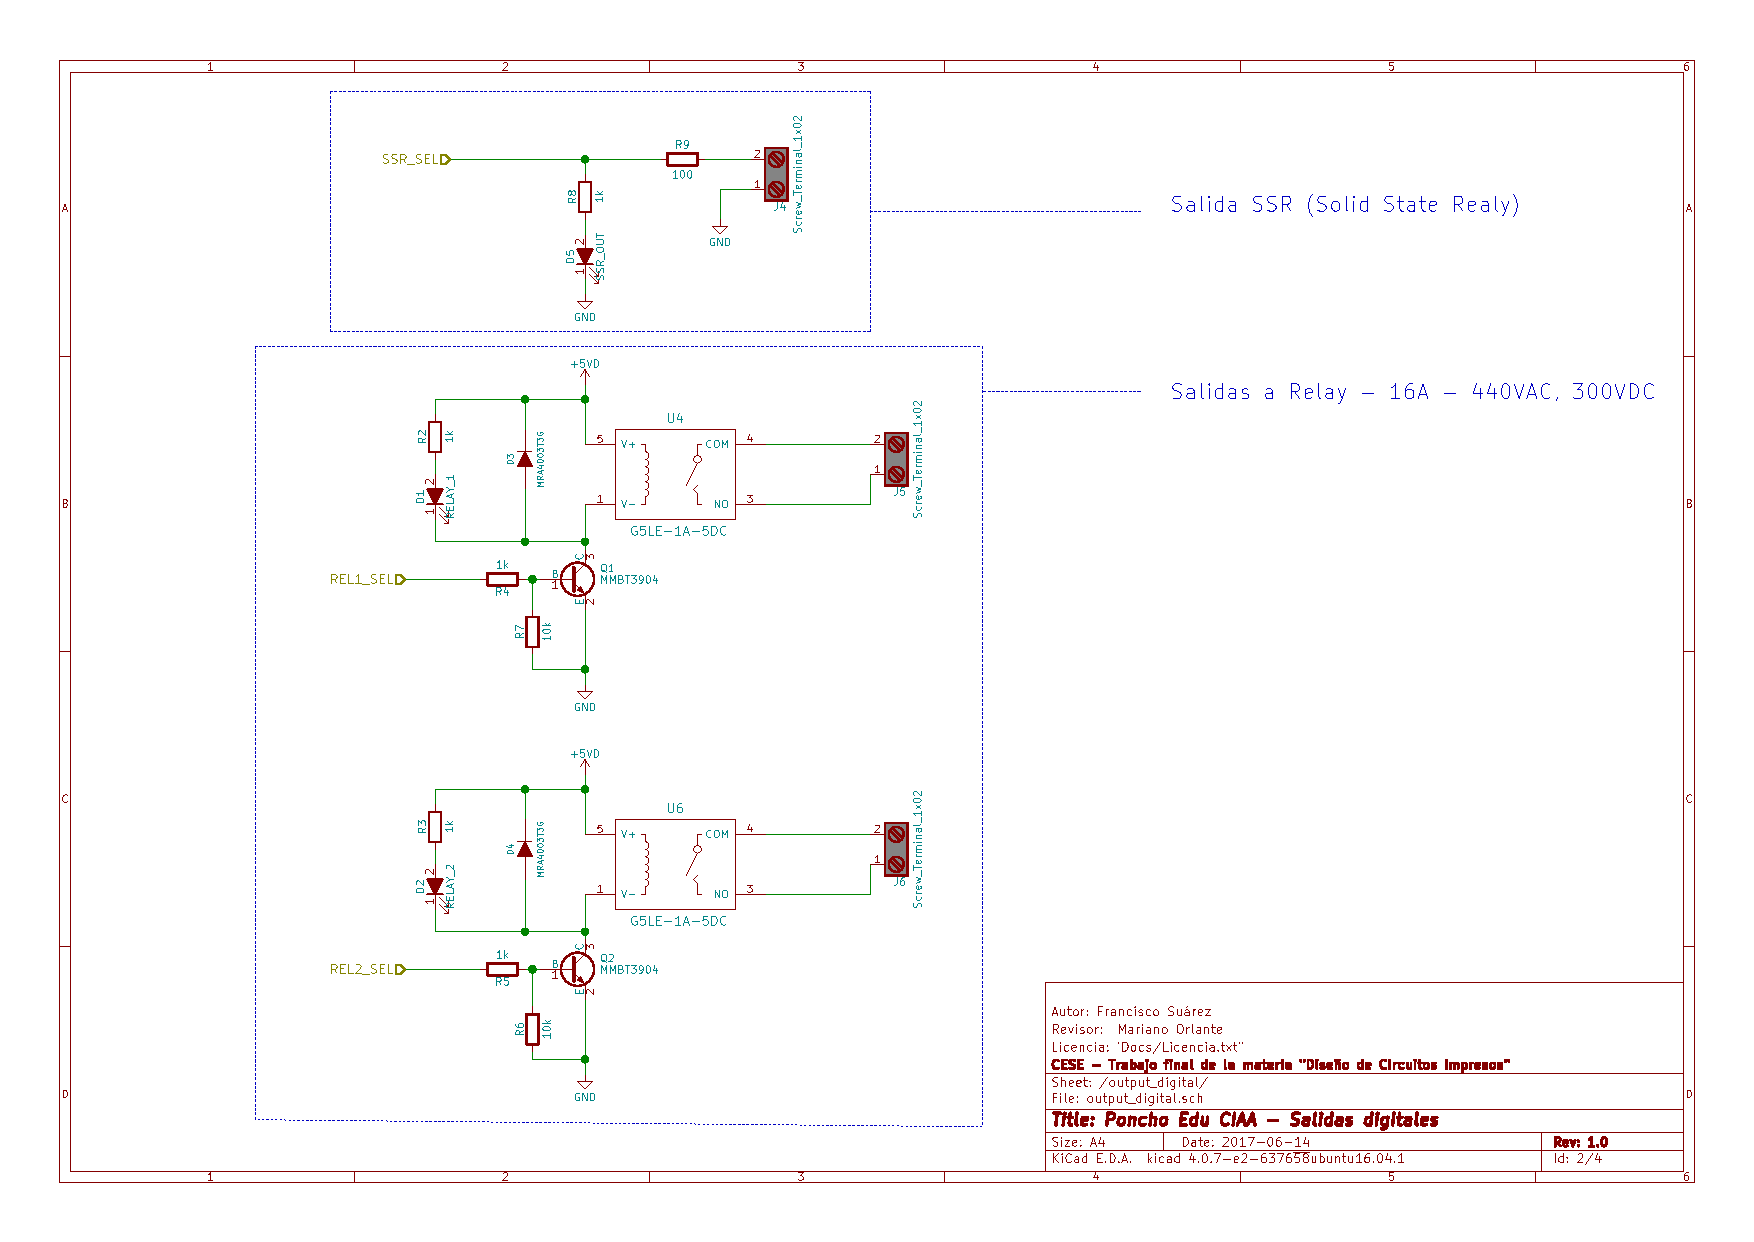
\includegraphics[width=1\textwidth]{Figures/Appendices/sch_outAnalogDigital}
	\caption{Esquemático de salidas digitales con relays.}
	\label{fig:schSalidas}
\end{sidewaysfigure}

\begin{sidewaysfigure}[h!]
	\centering
	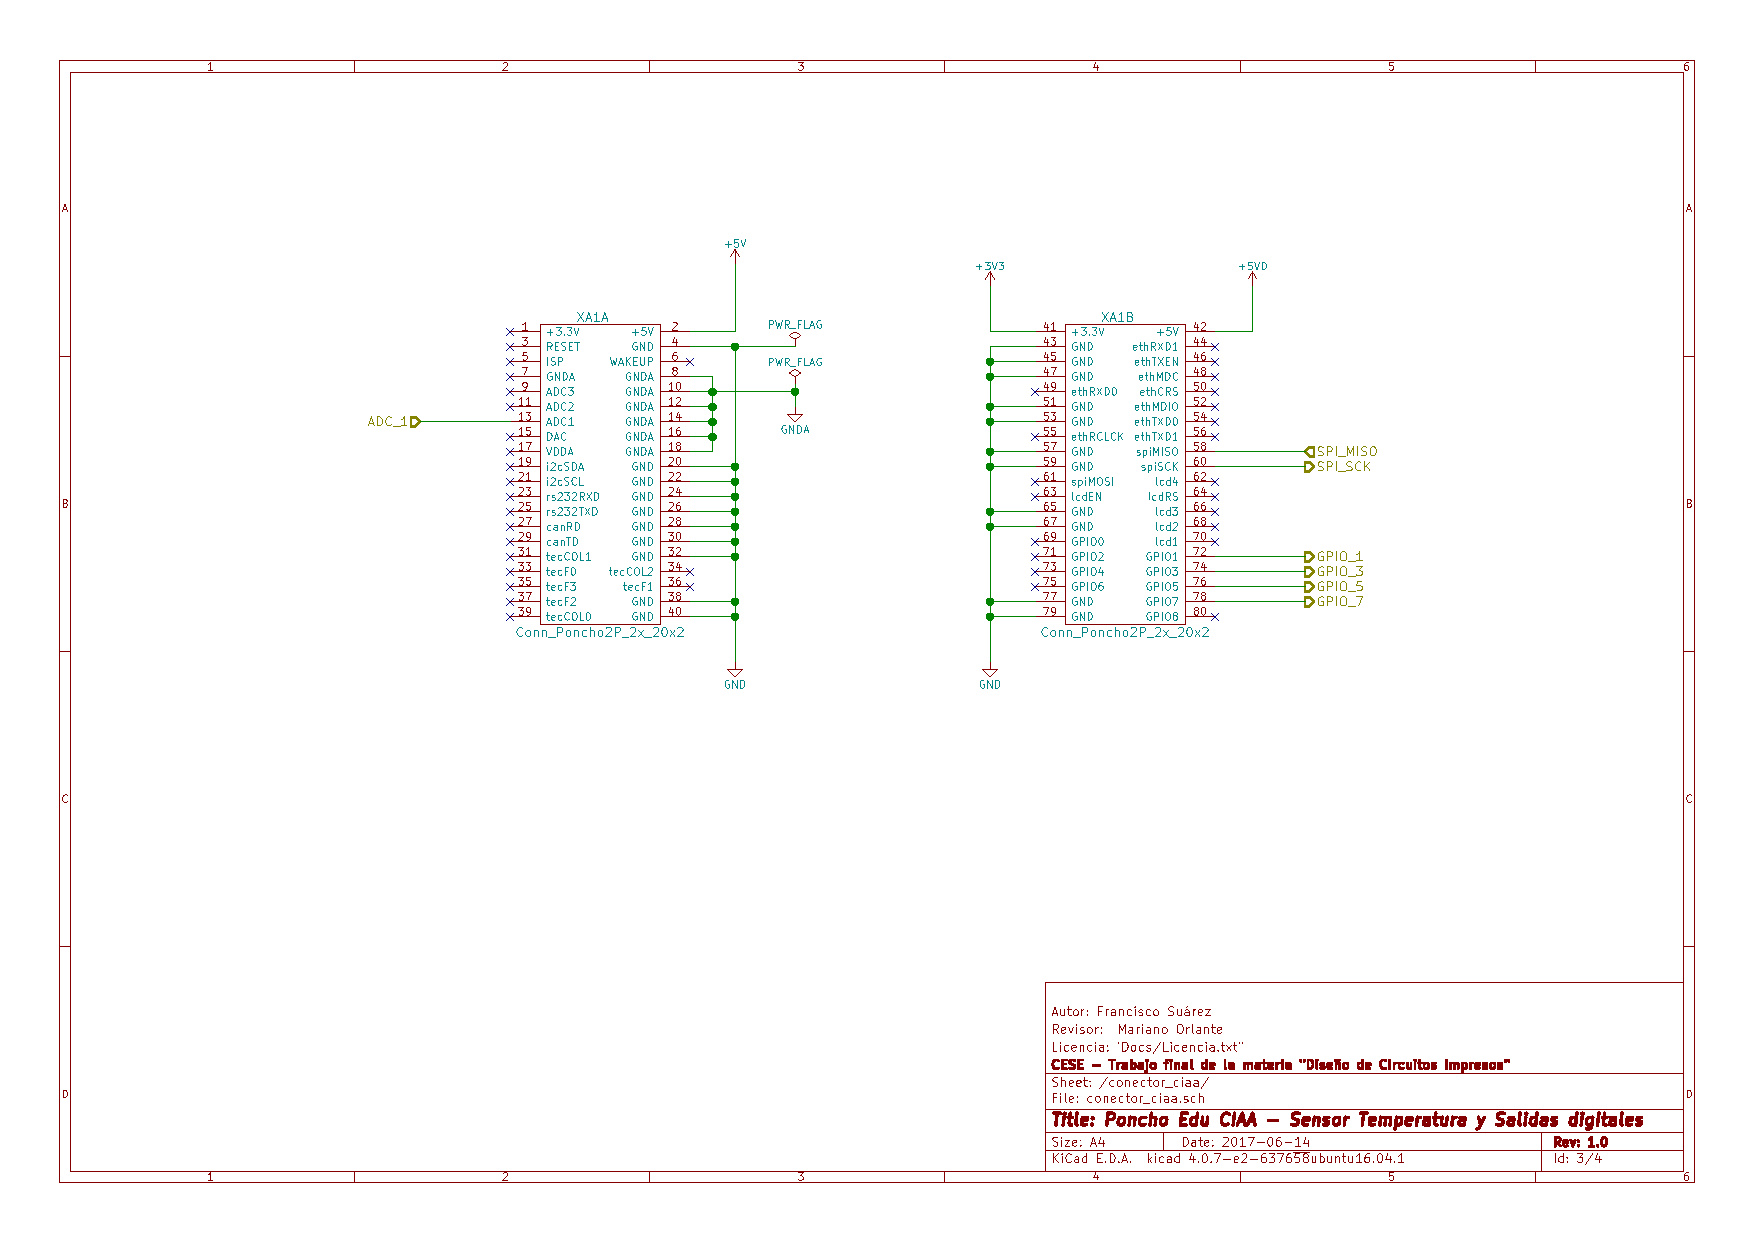
\includegraphics[width=1\textwidth]{Figures/Appendices/sch_conect_ciaa}
	\caption{Esquemático de conectores de expansión con la eduCIAA.}
	\label{fig:schSalidas}
\end{sidewaysfigure}



%% Appendix Template

\chapter{ Requerimientos Funcionales y no Funcionales } % Main appendix title

\label{AppendixC} % Change X to a consecutive letter; for referencing this appendix elsewhere, use \ref{AppendixX}

\begin{enumerate}

\item Requerimientos Funcionales
\begin{enumerate}

\item Temperatura (RFTEM)
\begin{enumerate}
\item El sistema medirá la temperatura con un resolución de XX, cada YY segundos.
\item El sistema mantendrá la temperatura controlada según los parámetros configurados por el usuario.
\item El sistema elevará la temperatura a través de la activación de una salida digital conectada a una resistencia.
\item La activación de la resistencia se implementará a través de una ventana Smith Trigger para evitar la intermitencia y generación de ruido en las líneas de alimentación principal. Cruce por 0.
\item En caso de que la temperatura se exceda de rango de considerar interrumpir el proceso y emitir una alarma.
\item El sistema almacenará al menos XX valores de temperatura en un archivo en memoria flash.
\end{enumerate}

\item Energía (RFENE)
\begin{enumerate}
\item El software medirá la corriente total (DC) entregada al proceso de electrólisis cada XX segundos, con YY de resolución.
\item El software medirá la tensión aplicada (DC) entre los bornes del electrólisis cada XX segundos con YY de resolución.
\item El sistema almacenará al menos XX valores de corriente y tensión en un archivo en memoria flash.
\item Los rangos de valores óptimos de tensión y corriente serán tomados de los parámetros de lote ingresados por el usuario y mostrados por pantalla para su configuración manual en la fuente de alimentación principal.
\end{enumerate}

\item Conductividad (RFCOND)
\begin{enumerate}
\item El software calculará a través de la corriente y tensión medidas en el tanque de galvanización, la conductividad de la solución salina cada XX segundos con YY de resolución.
\item El software deberá compensar las eventuales desviaciones de la conductividad óptima a través de la activación de XX válvulas de aditivos.
\end{enumerate}

\item Interfaces Hombre-Máquina (RFHMI)
\begin{enumerate}
\item El sistema contará con una pantalla estado del sistema con variables a definir.
\item El sistema contará con un método de ingreso de parámetros de lote a procesar.
\item Deberá permitir ingresar parámetros en modo manual y otros en modo codificado.
\item Deberá brindar a través de una interfaz Ethernet los históricos almacenados en memoria flash de variables del proceso que necesiten ser auditadas tras una etapa o tras el proceso completo. El máximo de registros será de XX número de puntos en formato YY.
\end{enumerate}

\begin{enumerate}
\item Tiempos (RFTI)
\item El software llevará un conteo del tiempo entre cada baño en las bateas, desde el momento que se inicia hasta el final del proceso.
\item En cada etapa deberá avisar y esperar a que un operario habilite la iniciación de la siguiente etapa.
\end{enumerate}

\item Niveles de bateas (RFNB)	
\begin{enumerate}
\item Evaluará que los niveles dentro del galvanizador estén dentro de los rangos permitidos de operación.
\item En caso de algún nivel crítico se emitirán alarmas y se considera la interrupción del proceso.
\end{enumerate}
\end{enumerate}

\item Requerimientos de Interfaz
\begin{enumerate}

\item Temperatura (RITEM)
\begin{enumerate}
\item La temperatura será medida a través de un sensor analógico de tolerancia XX.
\item La temperatura se medirá en los tanques XX, lo que arroja un total de YY numero de entradas analógicas independientes.(+xxAI)
\end{enumerate}

\item Energía (RIENE)
\begin{enumerate}
\item Tendrá un sensor de alta corriente del tipo XX conectado en una entrada analógica, para la corriente de galvanizador. (+1AI)
\item Tendrá un sensor de tensión de tipo XX conectados a los bornes de galvanizador. (+1AI)
\end{enumerate}

\item Conductividad (RICOND)
\begin{enumerate}
\item Tendrá XX dispositivos dosificador/es conectados a salidas digitales. (+xxDO)
\end{enumerate}

\item Interfaces Hombre-Máquina (RIHMI)
\begin{enumerate}
\item Debe mostrar información a través de un puerto VGA/HDMI con una taza de refresco menor a XX segundos. (+1USB)
\item Tomará de una entrada serie USB los valores de lote. (+1USB)
\item Accionara a través de una salida digital una alarma sonora/lumínica en caso de algún tipo de falla. (+1DO, +1AO) 
\item Contará con uno o dos pulsadores a fin de poder detener y accionar el procesos de galvanización, conectados a una/dos entradas binarias.(+1/2DO)
\item Dispondrá de una conexión remota a través de Ethernet. (+1ETH)
\end{enumerate}

\item Niveles de bateas (RINB)
\begin{enumerate}
\item Tendrá XX sensores de nivel conectados a entradas digitales. (+xxDI)
\end{enumerate}

\end{enumerate}

\item Requerimientos no Funcionales (RNF)
\begin{enumerate}
\item Deberá ser probada la funcionalidad a través de un banco de pruebas que se ajuste al comportamiento del sistema. 
\end{enumerate}

\item Restricciones de Diseño (RD)
\begin{enumerate}
\item De los requerimientos de interfaz se resume que como mínimo el hardware deberá contar con las siguientes interfaces:
Entradas analógicas:(AI) >= 3	\\
Entradas digitales: (DI) >= 3	\\
Salidas analógicas: (AO) >= 1	\\
Salidas digitales:  (DO) >= xx	\\
Puerto USB:	  		(USB)  = 2	\\
Puerto RED:	  		(ETH)  = 1	\\
\end{enumerate}

\item Requerimientos a Futuro (RAF)
\begin{enumerate}
\item Brindar información acerca de si es necesario realizar una limpieza de sistema. Se puede utilizar como parámetro el número de procesos que se ejecutaron 	 	 	
\item Deberá permitir loguearse antes de iniciar el proceso, así tener un responsable de operación.
\item Deberá interactuar con una cinta de transportación automática que llevará las placas de una batea a otra. Accionara los motores (paso a paso?) de transporte y de elevación.
\item Si no se respetan los tiempos el sistema deberá dejar asentado el técnico y las acciones manuales ejecutadas a fin de tener un histórico antes posibles fallas en el lote.
\end{enumerate}


%----------------------------------------------------------------------------------------
%	BIBLIOGRAPHY
%----------------------------------------------------------------------------------------

\Urlmuskip=0mu plus 1mu\relax
\raggedright
\printbibliography[heading=bibintoc]

%----------------------------------------------------------------------------------------

\end{document}  
